\documentclass[12pt]{article}

% Load packages and define formatting options
\usepackage{geometry}
\usepackage{setspace}
\usepackage{titlesec}
\usepackage{times}
\usepackage{indentfirst}
\usepackage{scalerel}
\usepackage{float}

\edef\restoreparindent{\parindent=\the\parindent\relax}
\usepackage{parskip}
\restoreparindent

\usepackage{graphicx}
\graphicspath{{./Figures/}}

\usepackage{amsmath}
\numberwithin{equation}{section}
\numberwithin{figure}{section}
\numberwithin{table}{section}
\bibliographystyle{aiaa}

\geometry{margin=1in}
\onehalfspacing

\titleformat{\subsection}
  {\normalfont\fontsize{14}{16}\selectfont}{\thesubsection}{1em}{}

\setcounter{secnumdepth}{3}

\setlength{\abovedisplayskip}{0pt}
\setlength{\abovedisplayshortskip}{0pt}
\setlength{\belowdisplayskip}{0pt}
\setlength{\belowdisplayshortskip}{0pt}

\begin{document}

% Title Page
\setcounter{page}{1}
\pagenumbering{roman}
\begin{titlepage}
    \centering
    \vspace*{3cm}
    {\fontsize{28}{32}\selectfont \textbf{Guidance Algorithm for an Atmospheric Re-entry Vehicle}}
    \vfill
    a project presented to \\
    The faculty of the Department of Aerospace Engineering\\
    San Jose State University\\
    \vfill
    in partial fulfillment of the requirements for the degree\\
    {\fontsize{14}{16}\selectfont \emph{\textbf{Master of Science in Aerospace Engineering}}}\\
    \vfill
    by\\
    {\fontsize{18}{20}\selectfont \textbf{Arash Mehdipour}}\\
    February 2023\\
    \vfill
    {\fontsize{10}{12} \selectfont approved by}\\
    Dr. Thomas Lombaerts\\
    {\fontsize{10}{12} \selectfont Project Advisor}

\end{titlepage}

% Copyright Page
\newpage
\thispagestyle{empty}
\mbox{}
\vfill
\begin{center}
\emph{Copyright © [Year] by Your Name\\[0.2cm]
All Rights Reserved}
\end{center}
\newpage

% Abstract Page
\setcounter{page}{3}
\section*{\centering ABSTRACT}


\newpage

% Acknowledgements Page
\section*{Acknowledgements}


\newpage

% Table of Contents
\tableofcontents

\newpage

% List of Figures
\listoffigures

\newpage

% List of Symbols
\section*{List of Symbols and Acronyms}
\vfill
\begin{center}
\begin{tabular}{|c|c|c|}
\hline
\textbf{Symbols} & \textbf{Definition} & \textbf{Units} \\
\hline
Angle of Attack & $\alpha$ & radians\\
\hline
Side-slip Angle & $\beta$ & radians\\
\hline
Pitch Angle & $\theta$ & radians\\
\hline
Roll Angle & $\phi$ & radians\\
\hline
Yaw Angle & $\psi$ & radians\\
\hline
Flight Path Angle & $\gamma$ & radians\\
\hline
Bank Angle & $\sigma$ & radians\\
\hline
Planetary Rotation Rate & $\Omega$ & rad/s\\
\hline
Semi-major Axis & a & km\\
\hline
Semi-minor Axis & b & km\\
\hline
Eccentricity & e & N/A\\
\hline
Flattening & f & N/A\\
\hline
Normal Radius of Curvature & $R_n$ & km\\
\hline
Meridian Radius of Curvature & $R_m$ & km\\
\hline
Geodetic Latitude & $L$ & radians\\
\hline
Geocentric Latitude & $\Phi$ & radians\\
\hline
Longitude & $\lambda$ & radians\\
\hline
Geodetic Altitude & h & km\\
\hline
Gravity & g & m/s$^2$\\
\hline
Gravitational Constant & $\mu$ & km$^3$/s$^2$\\
\hline
Rotation Matrix & $C$ & N/A\\
\hline
Mass & m & kg\\
\hline
Inertia Tensor & $J$ & kg$\cdot$m$^2$\\
\hline
Drag Force & $D$ & N\\
\hline
Lift Force & $L$ & N\\
\hline
Side Force & $S$ & N\\
\hline
Body Roll Rate & $p$ & rad/s\\
\hline
Body Pitch Rate & $q$ & rad/s\\
\hline
Body Yaw Rate & $r$ & rad/s\\
\hline
Rolling Moment & $\mathcal{L}$ & N$\cdot$m\\
\hline
Pitching Moment & $\mathcal{M}$ & N$\cdot$m\\
\hline
Yawing Moment & $\mathcal{N}$ & N$\cdot$m\\
\hline

\hline
Altitude & alt & km\\
\hline
Velocity & V & km/s\\
\hline
& &\\
\hline
\textbf{Acronyms} & &\\
\hline
RV & Re-entry Vehicle & N/A\\
\hline
DEV & Deployable Entry Vehicle & N/A\\
\hline
ADEPT & Adaptable, Deployable, Entry and Placement Technology & N/A\\
\hline
LNA & Lifting Nano ADEPT & N/A\\
\hline
IMU & Inertial Measurement Unit & N/A\\
\hline
INS & Inertial Navigation System & N/A\\
\hline
GPS & Global Positioning System & N/A\\
\hline
NDI & Non-linear Dynamic Inversions & N/A\\
\hline
INDI & Incremental Non-linear Dynamic Inversion & N/A\\
\hline
LEO & Low Earth Orbit & N/A\\
\hline
ECEF & Earth Centered Earth Fixed & N/A\\
\hline
MCMF & Mars Centered Mars Fixed & N/A\\
\hline
NED & North East Down & N/A\\
\hline
CFD & Computational Fluid Dynamics & N/A\\
\hline
CAD & Computer Aided Design & N/A\\
\hline
\end{tabular}
\end{center}
\vfill

\newpage
\setcounter{page}{1}
\pagenumbering{arabic}

% Main Body of Document
\section{Introduction}

\subsection{Motivation}
 Atmospheric re-entry presents many challenges to the designers of a re-entry vehicle (RV). The high Mach numbers encountered during re-entry leads to large amounts of heat flux into the structure of the of the RV, which, if not properly accounted for, can cause catastrophic damage to the vehicle, leading to failure of the mission and, as seen with the space shuttle Columbia, even the death of the crew [1]. Since the heating of the RV is caused by the high Mach numbers typically seen during re-entry, there is also a need to quickly decelerate the vehicle to reduce the thermal loads encountered. For most RVs, this is typically achieved by using drag to decelerate the vehicle, which means that there is also a requirement for the sizing of the frontal area of the RV so that the desired deceleration can be met. The frontal area and deceleration requirements can cause the RV to be much larger than it needs to be in some cases, relative to the size of the payload it is delivering. Additionally, the larger area and nose radius of the windward surface helps with the thermal load management of the vehicle. This can not only lead to increased costs, but the larger RV produces packaging challenges to the launch vehicle, and can sometimes dictate that the launch vehicle be larger than it needs to be.

To help combat this problem, a stowable heat shield that can be loaded in a compact manner and then deployed during re-entry was developed. These systems are referred to as Deployable Entry Vehicles (DEVs), and have the benefits of reduced volume and mass when compared traditional rigid heat shields. The reduced mass in conjuction with the ability to be stowed in a compact form, allows for larger and heavier payloads to be stored within the launch vehicle. Additionally, the DEV concept allows for a modular heat shield system that can be attached to many different forms of payloads, easing the design time and cost for payload manufacturers. The Adaptable, Deployable, Entry and Placement Technology (ADEPT) vehicle is a DEV designed by NASA which features a "mechanically deployable low-ballistic coefficient aeroshell" [2] and is the vehicle for which the guidance algorithm in this paper will be developed.

Guided re-entry provides many benefits. In cases where the RV is returning to Earth, guided entry can allow the RV to land in a specified location, allowing the operators to easily and safely recover the RV and its payload. Additionally, this avoids safety hazards that an unguided RV may encounter, as exclusion zones around populated areas or other nation's territories can be programmed into the vehicle. In situations where a payload is sent to other celestial bodies, such as the Moon or Mars, a guided vehicle can land the payload close to a point of interest, reducing the time a rover or similar vehicle would need to travel before it can start collecting data. A guided RV is also able to control its speed through the atmosphere, thus having more control over the aerothermal loads the payload and heat shield experience, potentially leading to less ablative material being required for the heat shield and thus reducing cost and mass. The guidance system also provides the benefit of controlling the maximum deceleration rate, which is beneficial if the payload contains a human crew that needs to reach the surface safely. Therefore, a guidance algorithm is proposed for the ADEPT re-entry vehicle that will guide the RV to a specified location on the surface of a planet, while meeting constraints on maximum allowable deceleration and maximum temperature of the payload.

\subsection{Literature Review}
The proposed guidance system will be developed for a variant of ADEPT known as the SR-1. The SR-1 variant features a 0.7m deployable carbon fabric heatshield, that unfolds along 8 ribs that are positioned in a 70$^\circ$ symmetric pattern along the shield, similar to an umbrella [3]. The SR-1, seen on the left in Figure 1.1 below, was tested as the payload for a SpaceLoft XL SR sounding rocket launched from White Sands Missile Range in New Mexico. The SR-1 performed a chuteless descent and was able to recovered without incident thanks to the installation of a GPS receiver and C-band transponder, which are technologies that can be leveraged for Earth based missions. The inclusion of a GPS receiver means that GPS can also be used as an aiding source for the RV's navigation system for missions where a payload may need to be returned from orbit or from the Moon back down to Earth's surface safely. NASA is currently aiming to expand the ADEPT and DEV concepts to perform large payload delivery to Mars, Venus, and Saturn's moon, Titan.

\begin{figure}[h]
  \centering
  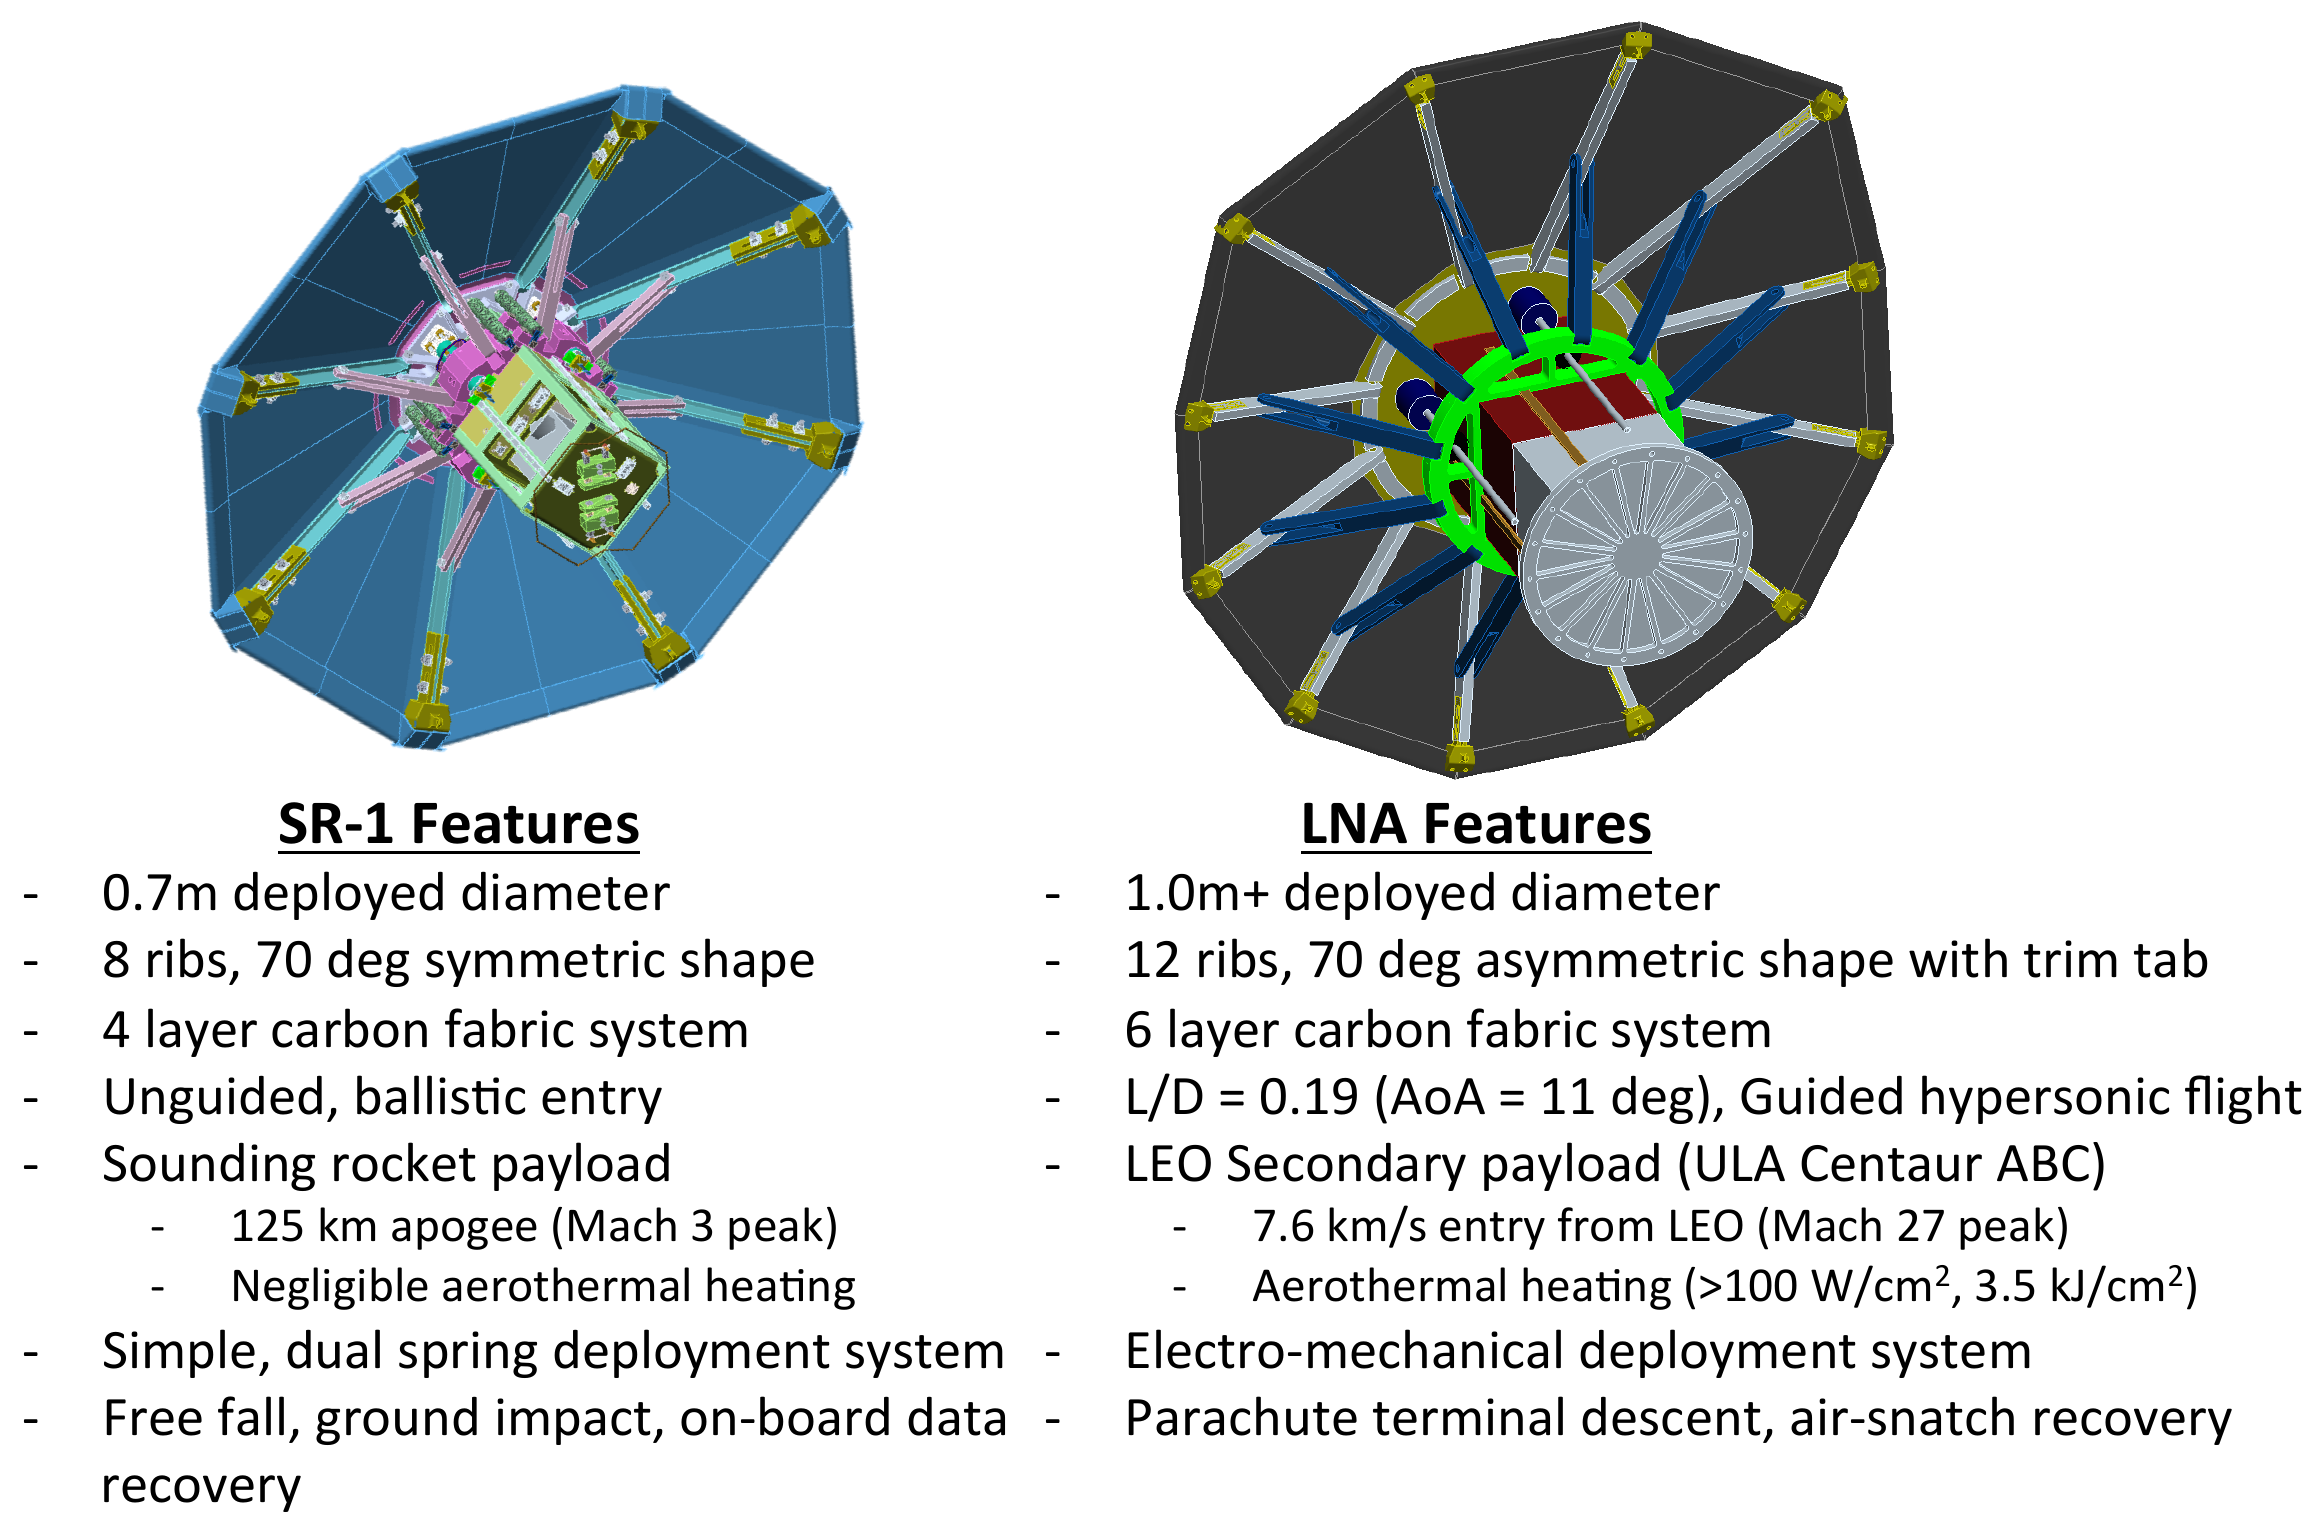
\includegraphics[width=0.7\textwidth]{SR-1 LNA Specs LNA Vehicle Concept.png}
  \caption{SR-1 and LNA vehicle features [3]}
  \label{fig:SR1_LNA}
\end{figure}

\begin{figure}[h]
  \centering
  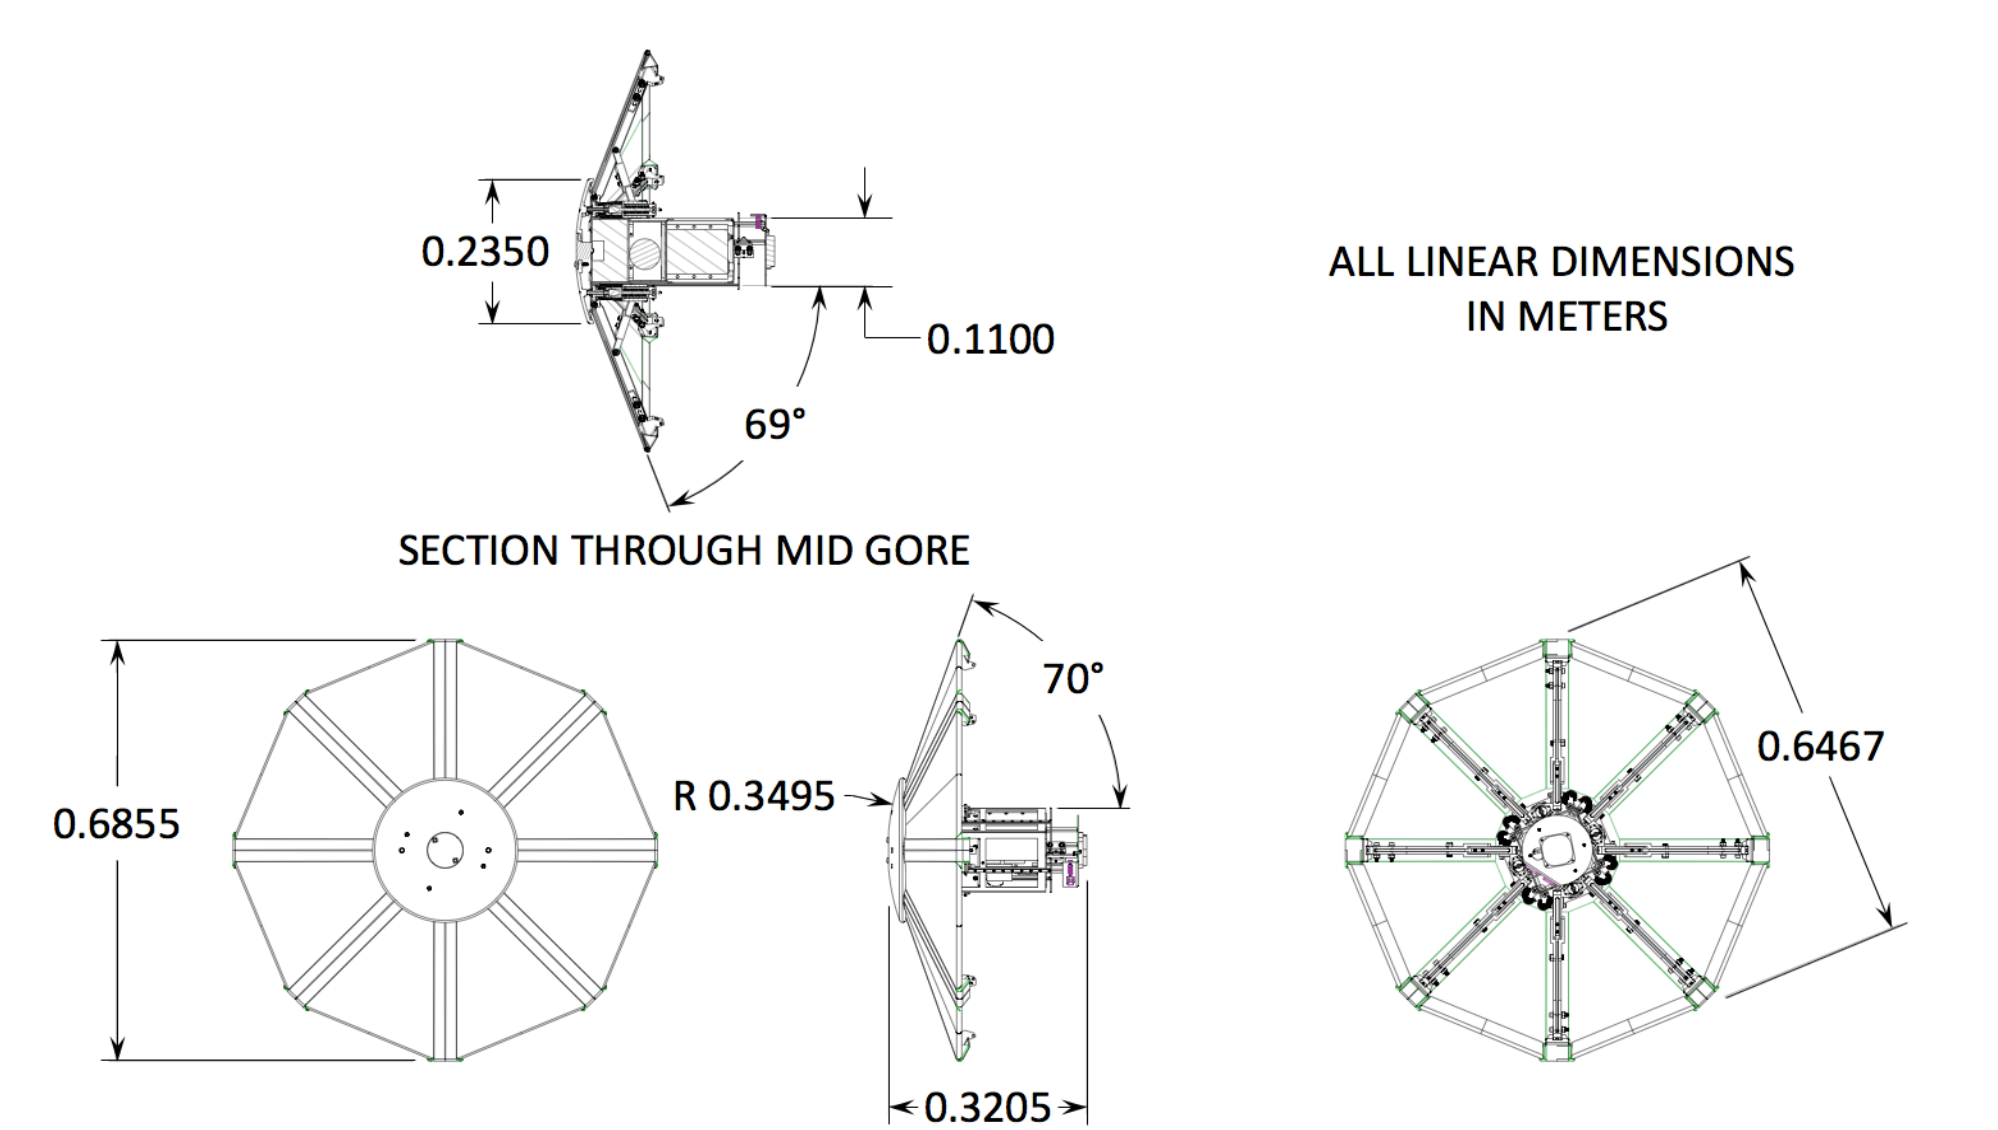
\includegraphics[width=1\textwidth]{Figures/SR-1 Dimensions Subsonic Dynamic Testing.png}
  \caption{Dimensions of the SR-1 [4]}
  \label{fig:SR1_Dims}
\end{figure}

\begin{table}
\begin{center}
\caption{SR-1 Mass Properties [4]}
\begin{tabular}{|c|c|c|}
\hline
\textbf{Property} & \textbf{Value} & \textbf{Units} \\
\hline
Rib to rib diameter & 0.7 & m\\
\hline
Reference area & 0.3489 & $m^2$\\
\hline
Center of mass & [-109.80, 0.25, 0.25] & mm\\
\hline
Mass & 8.49 & kg\\
\hline
$I_{xx}$ & 0.25 & kg$\cdot m^2$\\
\hline
$I_{yy}$ & 0.1722 & kg$\cdot m^2$\\
\hline
$I_{xx}$ & 0.1719 & kg$\cdot m^2$\\
\hline
\end{tabular}
\end{center}
\end{table}

The SR-1 vehicle was chosen as the development vehicle as a control system has already been developed for it in [5], as well as a CFD analysis to obtain all relevant aerodynamic values and coefficients. Control authority is provided through the use of 8 flaps that are placed at the end of each rib which can be seen in Figure 1.3, along with the body axis coordinate system definition for the vehicle. Pitch control is managed by flaps 2, 3, 6, 7 and yaw control is handled by flaps 1, 4, 5, and 8 [5]. Two control laws were developed for the SR-1 in [5], one law utilizing non-linear dynamic inversion (NDI), and the other using a modification of NDI known as incremental non-linear dynamic inversion (INDI). While NDI has the benefits of allowing linear control system architectures to be applied to non-linear systems, it relies heavily on the fidelity of the system model used. Therefore, modelling errors and uncertainties can negatively impact the robustness and effectiveness of the controller. The INDI method was developed to help reduce the negative effects of modelling errors on the controller, and is outlined in [6], where a INDI controller is developed and analyzed for a Cessna Citation Aircraft. Reference [7] shows that an INDI controller is still able to track an input command in the prescence of noise, when tuned correctly. A selection of test cases was run in [5] varying the initial Mach number from 20-30, and the initial altitude from 80-120km, and showed that the INDI and the NDI controllers have similar performance and are able to track pitch, angle of attack, and side-slip angle commands. A study was also performed in [5] where a 10\% error was applied to the input states of the controller, and it was shown that the INDI controller was more robust to modelling error in the form of a bias than the NDI controller.

\begin{figure}[h]
  \centering
  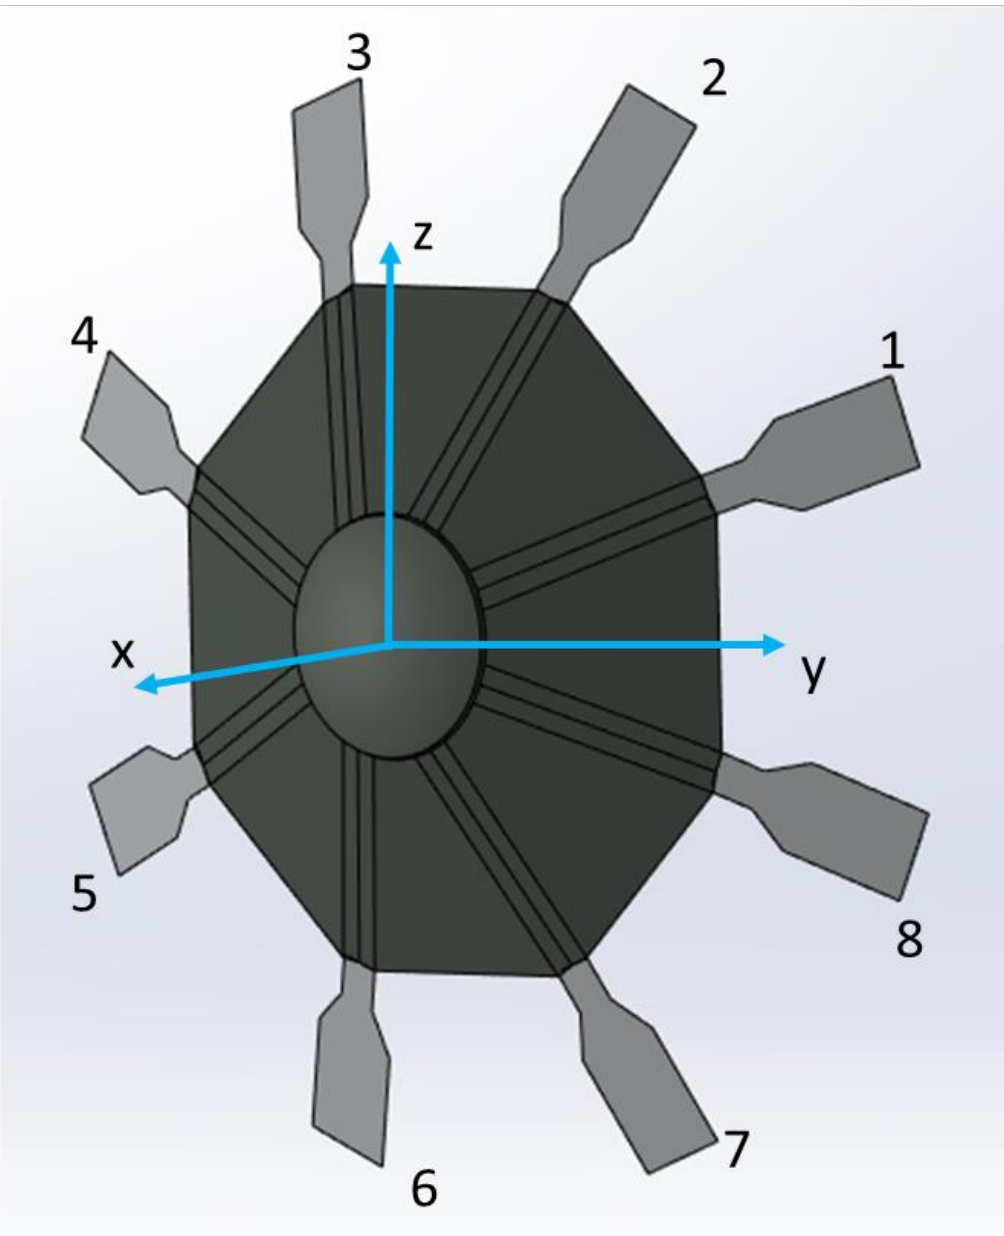
\includegraphics[width=0.3\textwidth]{Figures/SR-1 Controls and Coordinate.png}
  \caption{Attitude control flap layout of the SR-1 [5]}
  \label{fig:SR1_Controls}
\end{figure}

Understanding the system's performance in the presence of measurement noise is important, as in reality there exists no perfect sensors. In reality, the attitude rates and accelerations would be provided to the guidance and control algorithms by means of an IMU, which is subject to various sources of error and noise. MEMS gyroscopes and accelerometers are subject to biases, angular and velocity random walks, scale factor and misalignment errors, and temperature effects, the last of which is especially pertinent to a re-entry vehicle [8]. The errors on the acceleration and angular rate measurements cause issues for the navigation system as well, as the gyroscope measurement errors are integrated once to find the body attitude angles, and the accelerometer errors are integrated twice when calculating position. Integration of IMU errors causes the state estimates to drift over time, making it difficult to accurately control the RV and follow a prescribed trajectory. Additionally, while not considered "noise" in the sense of measurement noise such as with the IMU, other forms of noise can arise from a lack of fidelity of the system model. Unaccounted for sources such as manufacturing errors, damage, actuator dynamics errors, and flexible body dynamics amount to noise in the measured states versus the modeled states and need to be accounted for as well. The aforementioned sources of noise are typically called process noise in Kalman filtering [9]. Properly accounting for IMU and process noise normally requires the development of a Kalman filter and necessitates the use of aiding data such as GPS or a star tracker system [9]. An analysis of the guidance and control algorithm's sensitivity to measurement noise and bias is presented later in this paper.

Re-entry guidance began with the Apollo program, where a guidance algorithm was developed for a low-lifting capsule [10,11]. The Apollo algorithm consisted of two separate parts, one for the skip entry phase and one for the final entry phase. The algorithm used a pre-programmed trajectory and uses estimates of its own states to generate errors to the planned trajectory and make corrections. Since relatively poor computing performance was available in the days of the Apollo compared to today's standards, the algorithm relied mainly approximate, empirical, and analytical relationships with negatively impacted the performance of the guidance system [11]. The space shuttle used what is referred to as "second generation" guidance algorithms [11,12]. The shuttle, however, has a much higher lift to drag ratio than the ADEPT vehicles meaning that its guidance requirements are different due to the increased entry time caused by the larger L/D. When compared to Apollo, the space shuttle maintained a relatively small flight path angle, and defined a longitudinal trajectory using the acceleration due to drag and Earth-relative velocity when Mach numbers were high [11].

More modern methods leverage the increased computing power we have available today, and generate trajectories and guidance solutions online. Predictor-corrector methods are outlined in [11,15-17] and have become a modern choice for guidance for low lift RVs. Predictor-corrector methods do not rely on pre-planned trajectories and can do no require a separate trajectory planner and tracking law. A downside to early predictor-corrector methods was that they were unable to handle inequality constraints such as with heating constraints or aerodynamic loads. Reference [11] proposes this downside as the reason why the method is common for low lift RVs, as the heating and load constraints are generally satisfied by the initial entry conditions for those cases. The paper proposes an augmented algorithm that utilizes the quasi-equilibrium glide condition (QEGC) [13] to allow for predictor-corrector methods to satisfy heating and load constraints. Analyses conducted on vehicles that have 1/3 of the L/D of the space shuttle (similar to ADEPT), as well as the same L/D, and three times the L/D show that the augmented predictor-corrector algorithm is able to satisfy inequality constraints for a variety of RV types [11,13]. Even more modern methods, such as the one outlined in [18] leverage neural networks and machine learning to find patterns in re-entry data and generate commands based on the data.

Online generation of trajectories offers many benefits over traditional guided re-entry algorithms. Removing the dependency of a pre-determined trajectory allows the RV to respond dynamically and in real time to changing mission objectives or conditions. If the mission must be aborted, for whatever reason, the RV will be able to generate a new trajectory in real time to follow commanded abort parameters. Similarly, if the landing location of the RV needs to be changed mid-flight, the new location need simply to be told to the RV and a new trajectory to that location can be generated online. This also facilitates the use of dynamic exclusion zones and allows the vehicle to respond to otherwise unaccounted for situations. Therefore, an augmented predictor-corrector guidance algorithm such as the one outlined in [11,15-17] will be developed for the ADEPT SR-1. Sample initial entry conditions for a lunar return and an LEO return from [20] as initial test points. A Martian re-entry will be analyzed later in this paper. The heating constraints are defined in [3] as a maximum allowable of 200$\frac{W}{cm^2}$ and 4.5$\frac{J}{cm^2}$ for heat flux and heat load respectively. The proposed guidance algorithm will have to satisfy these constraints for various re-entry initial conditions and when alternate landing locations are specified mid-course. According to [21], humans can sustain a maximum of 12 gees of deceleration for short periods at a time, so the algorithm will also have to meet this constraint for manned missions.

\begin{table}
\begin{center}
\caption{ADEPT Sample Trajectories [20]}
\begin{tabular}{|c|c|c|c|}
\hline
\textbf{Property} & \textbf{Lunar Return} & \textbf{LEO Return} &  \textbf{Units}\\
\hline
Altitude & 122 & 122 & km\\
\hline
Velocity & 11.0 & 7.89 & km/s\\
\hline
$\gamma$ & -5.5 & -6.8 & degrees\\
\hline
\end{tabular}
\end{center}
\end{table}

\begin{figure}[h]
  \centering
  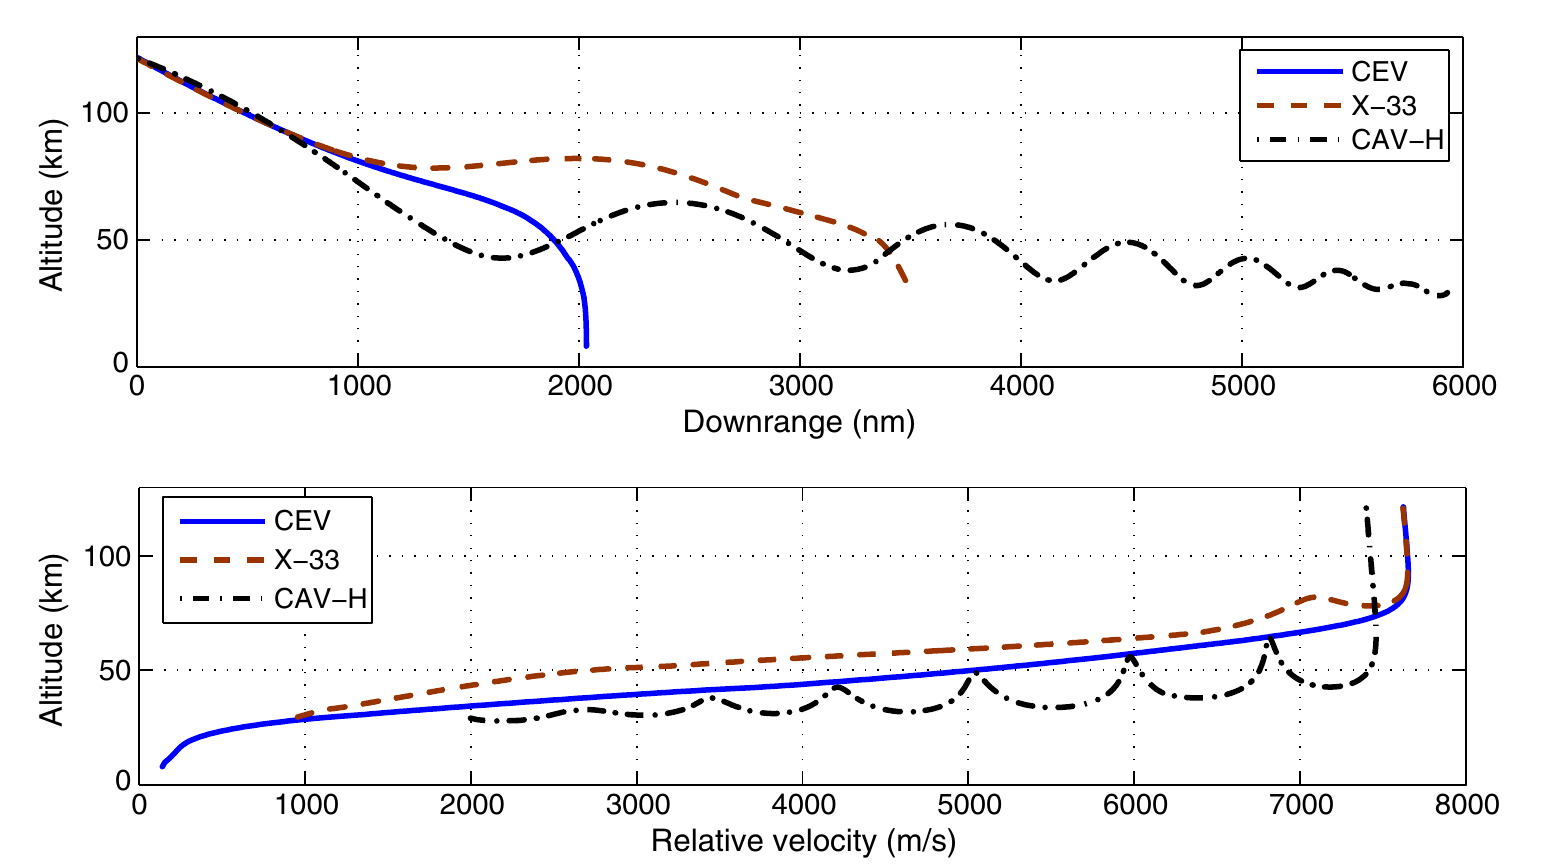
\includegraphics[width=1\textwidth]{Figures/different entry trajectories 11.png}
  \caption{Plots illustrating the different re-entry trajectories seen by a low-lift vehicle (CEV), a vehicle similar to the space shuttle (X-33), and a high L/S hypersonic glide vehicle (CAV-H) [11]}
  \label{fig:Reentry_Profiles}
\end{figure}

\subsection{Project Proposal}
The objective of this study is to develop a guidance algorithm for the ADEPT SR-1, building upon the control law developed in [5], that will allow the vehicle to be guided to a specified point on the surface, while meeting constraints on accuracy, heating load, and maximum deceleration. The algorithm will use modern augmented predictor-corrector methods found in [11,13,15-17] to generate trajectories online, and will be able to accept alternative landing point commands and guide itself to the new point. Additionally, a study will be conducted to assess the sensitivity of the guidance and control algorithms to measurement and process noise, and a filter constructed to account for the noise, if required.

\subsection{Methodology}
Mathematical models of the Earth and Mars atmospheres are constructed, as well as a method for calculating the chemical composition of the atmosphere based on the Mach number of the RV. This will facilitate the accurate calculation of the heat flux entering the RV and will be used as an input in the heat flux inequality constraint. Coordinate systems will be developed for both the Martian entry and the Earth return cases, to allow for navigation information to be fed into the guidance algorithm. An augmented predictor-corrector guidance law will be developed and tested in both entry environments, and its performance compared to the traditional method of pre-planned trajectories. Finally, a noise sensitivity analysis will be conducted for the controller and guidance algorithm, and a filter developed if necessary.

\section{Coordinate Frames and Transformations}
\subsection{Coordinate Frame Definitions}
Vehicle coordinate frames are defined as in Figure 2.1 below, with the ADEPT body axis frame constructed such that the x-axis points from the center of mass forward through the center of the deployable heat shield, the y-axis points from the center of mass to the right of the vehicle, and the z-axis points from the center of mass to the bottom of the vehicle. Additionally, a vehicle aerodynamic coordinate frame is defined around the velocity vector of the RV, and is achieved by rotation through the sideslip angle $\beta$, angle of attack, $\alpha$, and the aerodynamic roll angle, also known as the bank angle, denoted by $\sigma$.

\begin{figure}[h]
  \centering
  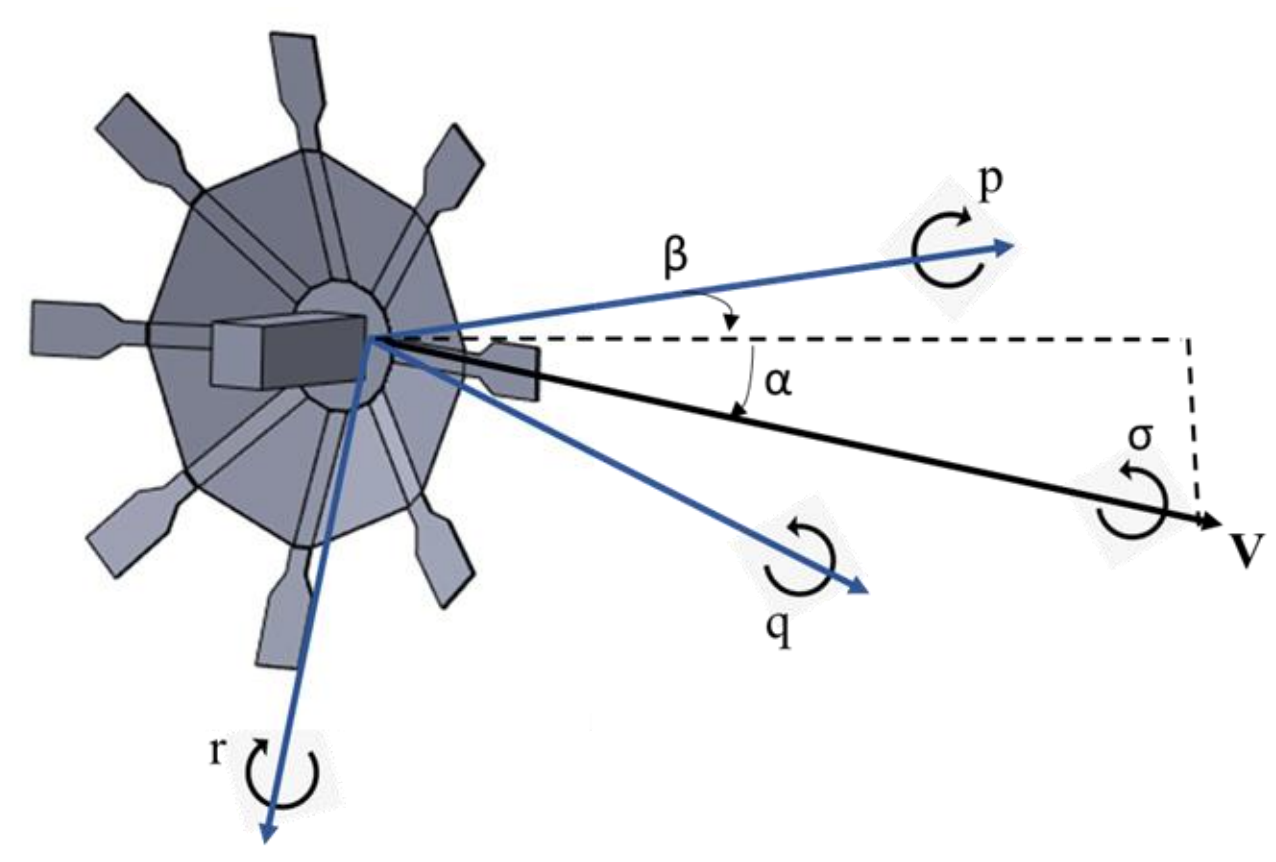
\includegraphics[width=1\textwidth]{Figures/Body_Frame_Angles.png}
  \caption{ADEPT vehicle aerodynamic frame angles and body rates [5]}
  \label{fig:Aero_angs}
\end{figure}

To describe the position of the ADEPT RV, additional coordinate frames must be defined for navigation purposes. The Earth-centered Earth-fixed coordinate frame, commonly refered to as ECEF, is a cartesian coordinate frame with its origin at the center of the Earth. The ECEF frame X axis points from the center of the Earth to the intersection of the equator and the prime meridian, the Y axis points from the center of the Earth to the intersection of the equator and the 90 degree meridian, and the Z axis points from the center of the Earth to the Earth's rotation axis with the positive direction pointing to true north. The ECEF frame is fixed with respect to the Earth, and thus rotates along with the Earth with a rotational speed $\omega_{Earth}$ of approximately 7.292115e-5 rad/s. For Mars based missions, a similar coordinate frame is defined, with the origin at the center of Mars and the axes pointing in the same directions as the ECEF frame. The Mars-centered Mars-fixed frame, denoted MCMF, is fixed with respect to Mars and rotates with a rotational speed $\omega_{Mars}$ of approximately 7.088218e-5 rad/s. The ECEF and Mars-fixed frames are used to describe the position of the RV with respect to the Earth and Mars respectively, and are useful when guiding the vehicle to a specified point on the respective planet's surface.

The reference ellipsoid for Earth is provided by the World Geodetic System 84 (WGS84). It defines the Earth semi-major axis, $a$, the semi-minor axis, $b$, and the flattening factor, $f$ as
\begin{gather*}
    \setlength\jot{-2ex}
    \begin{aligned}
        a &= 6378137.0\,\text{m} \\
        b &= 6356752.314245\,\text{m} \\
        f &= \frac{1}{298.257223563}
    \end{aligned}
\end{gather*}
respectively. The reference ellipsoid for Mars is provided by the Mars Orbiter Laser Altimeter (MOLA). It defines the Mars semi-major axis, semi-minor axis, and flattening factor as
\begin{gather*}
    \setlength\jot{-2ex}
    \begin{aligned}
        a &= 3396190.0\,\text{m} \\
        b &= 3376200.0\,\text{m} \\
        f &= \frac{1}{169.81}
    \end{aligned}
\end{gather*}
The flattening factor is used to define the eccentricity of the ellipsoid, $e$ and the first eccentricity squared, $e^2$, as
\begin{align}
    e &= \sqrt{2f - f^2},
\end{align}
\begin{align}
    e^2 &= 1 - {(1 - f)}^2.
\end{align}
The first eccentricity squared is then used to define the normal radius of curvature, $R_n$, and the meridian radius of curvature, $R_m$, as
\begin{align}
    R_n &= \frac{a}{\sqrt{1 - e^2\sin^2L}},
\end{align}
\begin{align}
    R_m &= \frac{a(1 - e^2)}{{(1 - e^2\sin^2L)}^{3/2}}.
\end{align}
where $L$ is the geodetic latitude of the point of interest.
The normal radius of curvature is used to define the normal gravity, $g_n$, as
\begin{align}
    g_n &= \frac{\mu}{R_n^2},
\end{align}
and the meridian gravity, $g_m$, as
\begin{align}
    g_m &= \frac{\mu}{R_m^2}.
\end{align}

\begin{figure}[h]
  \centering
  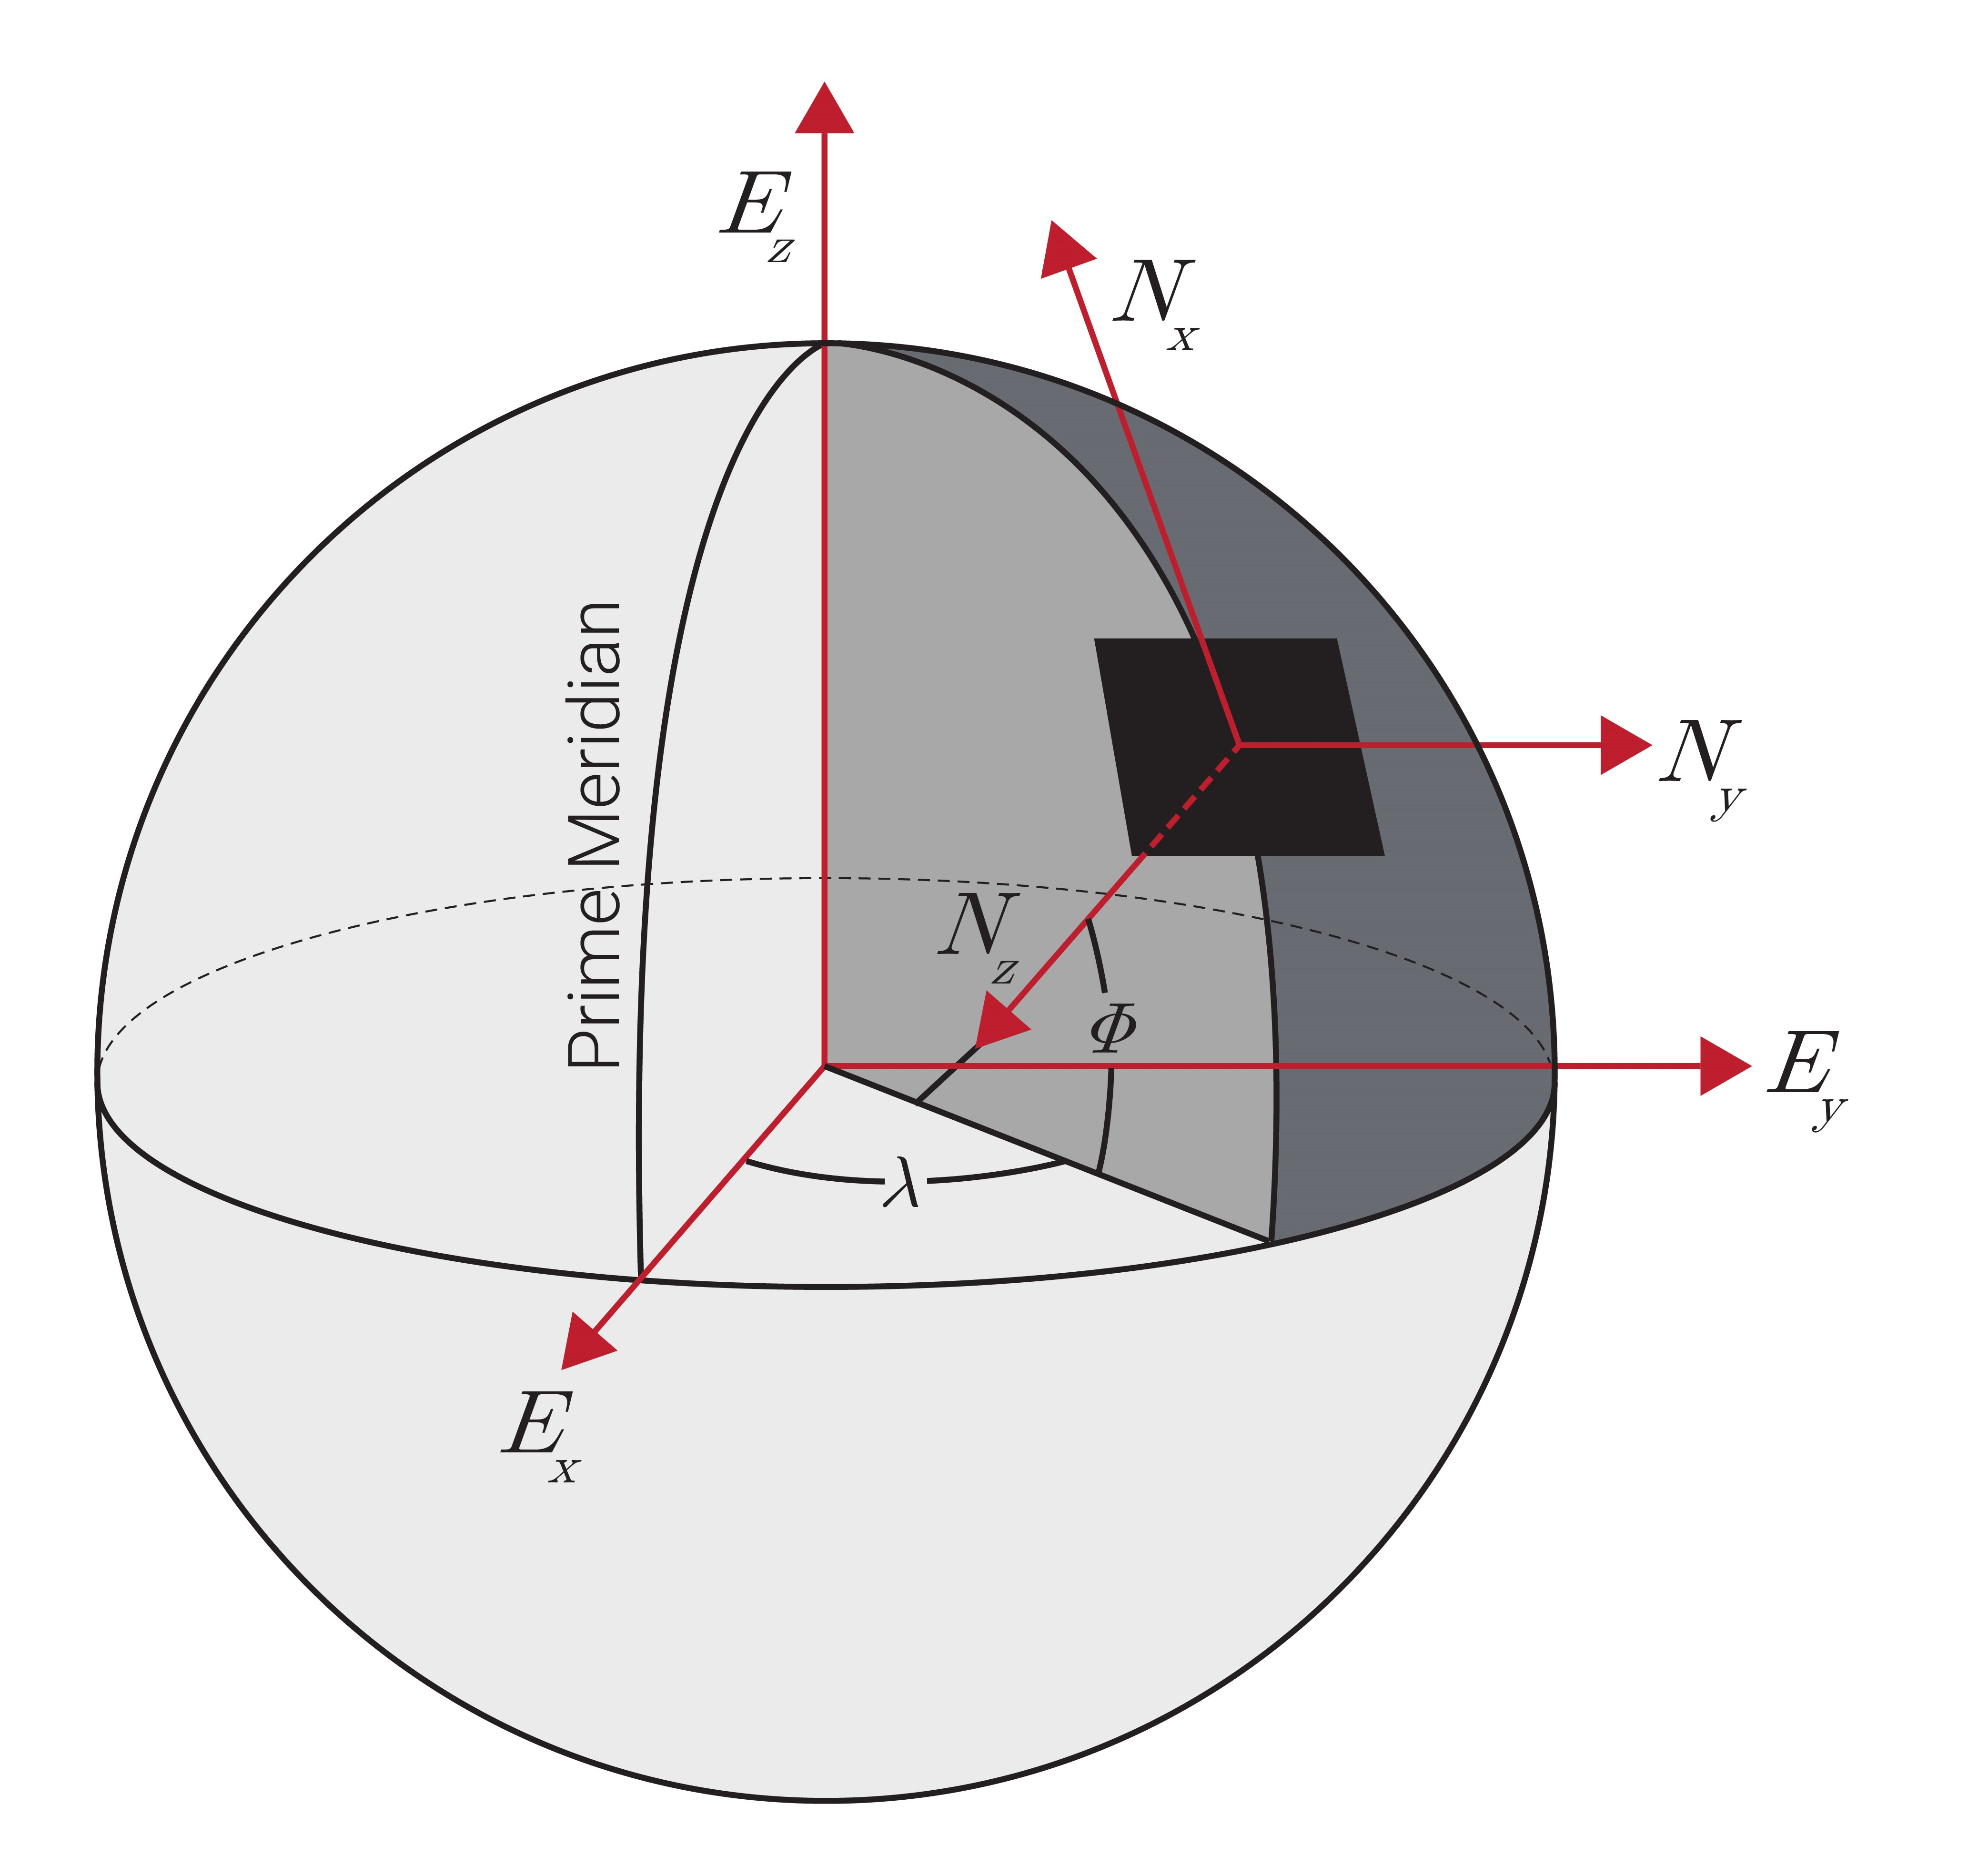
\includegraphics[width=0.5\textwidth]{Figures/ref_ecef.jpg}
  \caption{Illustration of the ECEF and NED coordinate frames. MCMF is constructed similarly to ECEF. [22]}
  \label{fig:ECEF}
\end{figure}

As a supplement to the ECEF and MCMF frames, two local level navigation frames are used for the guidance algorithm, the North-East-Down frame and the Wander Azimuth frame. The North-East-Down frame (NED) is a cartesian coordiante frame whose origin is generally either aligned with the center of gravity of the vehicle or attached to a point of interest. The NED frame is defined such that its X axis points towards true North, its Y axis points towards East, and its Z axis points down normal to the surface of the reference ellipsoid. The NED frame provides a more intuitive way to describe the position of the RV relative to points of interest than is provided by the ECEF or MCMF frames.


\subsection{Coordinate Frame Transformations}
Transformations between different coordinate frames are handled through the use of direction-cosine matrices (DCM). The DCM is a 3x3 matrix that transforms a vector from one coordinate frame to another and are denoted as $C^{^{\scaleto{A}{4pt}}}_{\scaleto{B}{4pt}}$ which reads in English as the rotation from coordinate frame B to coordinate frame A.
The transformation from the ECEF frame to the NED frame, $C^{^{\scaleto{NED}{4pt}}}_{\scaleto{ECEF}{4pt}}$ is achieved by first rotating through the longitude, $\lambda$ and then through the geodetic latitude, $L$ and is given by the equation
\begin{align}
  C^{^{\scaleto{NED}{4pt}}}_{\scaleto{ECEF}{4pt}} = \begin{bmatrix}
    -\sin L \cos {\lambda} & -\sin L \sin {\lambda} & \cos L \\
    -\sin {\lambda} & \cos {\lambda} & 0 \\
    -\cos L \cos {\lambda} & -\cos L \sin {\lambda} & -\sin L
  \end{bmatrix}
\end{align}

Similarly, the transformation between the body and NED frames is constructed through a 'Z-Y-X' rotation sequence through the body Euler angles, $\phi$, $\theta$, and $\psi$ and is given by the equation
\begin{align}
  C^{^{\scaleto{Body}{4pt}}}_{\scaleto{NED}{4pt}} = \begin{bmatrix}
    \cos{\theta}\cos{\psi} & \cos{\theta}\sin{\psi} & -\sin{\theta} \\
    \sin{\phi}\sin{\theta}\cos{\psi} - \cos{\phi}\sin{\psi} & \sin{\phi}\sin{\theta}\sin{\psi} + \cos{\phi}\cos{\psi} & \sin{\phi}\cos{\theta} \\
    \cos{\phi}\sin{\theta}\cos{\psi} + \sin{\phi}\sin{\psi} & \cos{\phi}\sin{\theta}\sin{\psi} - \sin{\phi}\cos{\psi} & \cos{\phi}\cos{\theta}
  \end{bmatrix}
\end{align}
and the rotation from the ECEF frame to the body frame is given by the equation
\begin{align}
  C^{^{\scaleto{Body}{4pt}}}_{\scaleto{ECEF}{4pt}} = C^{^{\scaleto{Body}{4pt}}}_{\scaleto{NED}{4pt}}C^{^{\scaleto{NED}{4pt}}}_{\scaleto{ECEF}{4pt}}
\end{align}
Earth was used as an example in the above equations, but the method is the same for Mars.

\section{Equations of Motion}
\subsection{Six Degree of Freedom Equations of Motion}
The following equations of motion of the ADEPT RV are taken from [19] and [23]. The linear dynamics are given by
\begin{align}
  \dot{V} &= -\frac{g(z)}{m}\sin\gamma - \frac{1}{m}D
\end{align}
\begin{align}
  \dot{\gamma} &= \biggl(-\frac{g(z)}{mV}\biggl)\cos\gamma + \frac{1}{mV}(L\cos\sigma - S\sin\sigma)
\end{align}
\begin{align}
  \dot\psi &= \frac{1}{mV\cos\gamma}(L\sin\sigma + S\cos\sigma)
\end{align}
where $V$ is the velocity of the RV, $\gamma$ is the flight path angle, $\psi$ is the heading angle, $g(z)$ is the gravitational acceleration at altitude $z$, $m$ is the mass of the RV, $D$ is the drag force, $L$ is the lift force, and $S$ is the side force.

The rotational dynamics are given by
\begin{align}
  \begin{bmatrix}
    \dot{p} \\
    \dot{q} \\
    \dot{r}
  \end{bmatrix} = J^{-1} \Biggl(\begin{bmatrix}
     \mathcal{L}\\
     \mathcal{M}\\
     \mathcal{N}
    \end{bmatrix}
    - \begin{bmatrix}
      p \\
      q \\
      r
    \end{bmatrix}
    \times J\begin{bmatrix}
      p \\
      q \\
      r
\end{bmatrix}
\Biggl)
\end{align}
where $p$, $q$, and $r$ are the roll, pitch, and yaw rates, respectively, $\mathcal{L}$, $\mathcal{M}$, and $\mathcal{N}$ are the roll, pitch, and yaw moments, and $J$ is the vehicle inertia tensor.

The translational kinematics are defined by
\begin{align}
  \dot{z} &= V\sin\gamma
\end{align}
\begin{align}
  \dot{\Lambda} &= \frac{V}{z}\cos\gamma\cos\psi
\end{align}
\begin{align}
\dot{\Phi} &= \frac{V}{z\cos\Lambda}\cos\gamma\sin\psi
\end{align}

and the rotational kinematics are defined by
\begin{align}
\dot{\sigma} = p\frac{\cos\alpha}{ \cos\beta} + r \frac{\sin\alpha}{\cos\beta}
\end{align}
\begin{align}
  \dot{\alpha} = -p\cos\alpha\tan\beta - r\sin\alpha\tan\beta + q
\end{align}
\begin{align}
\dot{\beta} = p\sin\alpha - r\cos\alpha
\end{align}

The figure below illustrates the the different quantities in the above equations are defined with respect to the ECEF and vehicle body frames. Note that the nomenclature differs between this paper and that used by the author of the image source. Notably, $\Phi$ as defined above is equivalent to $\lambda$, $\Lambda$ is equivalent to $\phi$, and $\psi$ is equivalent to $\xi$.

\begin{figure}[H]
  \centering
  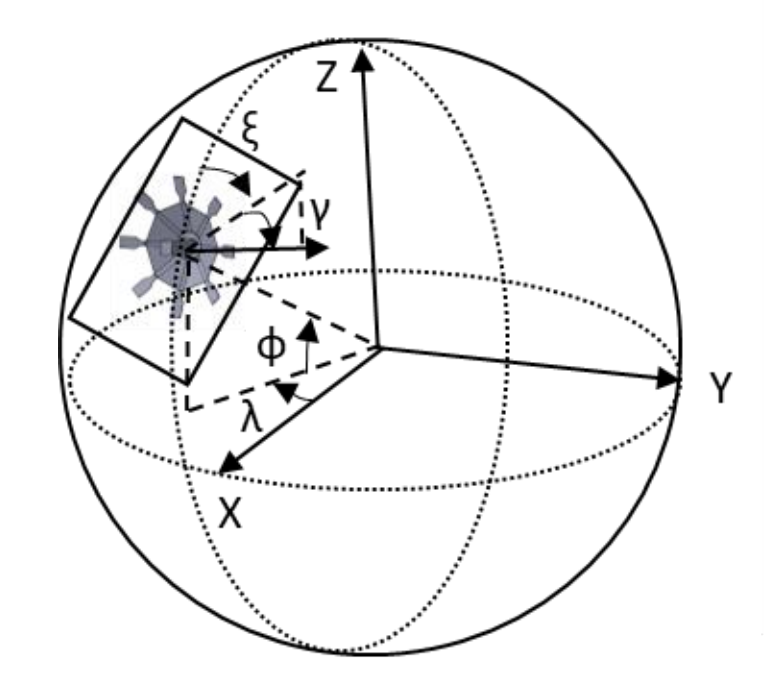
\includegraphics[width=0.5\textwidth]{Figures/ADEPT_Nav_Frame.png}
  \caption{Navigation coordinate frame definitions for the ADEPT vehicle [5]}
  \label{fig:ADEPT_Nav_Coordinate_Frames}
\end{figure}

Since a sufficiently small time step is used in the simulation, the equations of motion are integrated using a simple forward Euler integration scheme, where some quantity $x$ is integrated as $x_{i+1} = x_i + \dot{x}dt$ for each time step. The position of the ADEPT RV in the ECEF and NED frames are bookkept through the geodetic latitude and longitude, which are propagated at each time step through the following equations.

\begin{align}
L_{i+1} &= L_i + \frac{V_{N}}{R_m + z} dt
\end{align}
\begin{align}
\lambda_{i+1} &= \lambda_i + \frac{V_{E}}{(R_n + z)\cos(L_i)} dt
\end{align}

where $V_N$ and $V_E$ are the north and east components of the velocity vector, respectively, and $R_m$ and $R_n$ are the radii of the Earth in the meridional and normal directions, respectively.

\section{Simulation Studies}
\subsection{Noise Robustness Analysis}
In real world applications, guidance, navigation, and control (GNC) systems rely on information from sensors to perform their duties. However, sensors are not perfect and are subject to noise, biases, and scale factor and misalignment errors. Additionally, system modelling inaccuracies and unmodelled phenomena can appear as noise to GNC systems such as the controller. The NDI control scheme, in particular, relies heavily on the modeling fidelity of the system. Therefore, it is important to understand the effects of modelling and sensor noise on the system's performance and determine the robustness of the controller to ensure adequate performance in real world scenarious.

In [5] a test was conducted where the aerodynamic coefficients had a flat scaling factor applied to them to replicate the effects of modelling error. It was found that both the NDI and INDI control schemes, were robust the modelling errors in the form of scaling as can be seen in the figure below. In order to test the robustness of the ADEPT RV to sensor noise, simulations were performed where noise was added to the angular rate channels, $p, q, \text{and} r$, to simulate the effects of noise on the gyroscope measurements. The noise was added to the angular rate channels as a zero-mean Gaussian noise with a standard deviation ranging from $ \sqrt{1e-5}$ to $\sqrt{1e-3}$ rad/s. The results of the simulations can be seen in the figure below. It can be seen that both the NDI and INDI control schemes are robust to the noise in the angular rate channels up to a noise spectral density of 1e-3 rad/s. For the purposes of the guidance system design, it can be assumed that the NDI and INDI control schemes are robust to sensor noise and that an IMU with a noise spectral density of significantly less than 1e-3 rad/s is used.

\begin{figure}[H]
  \centering
  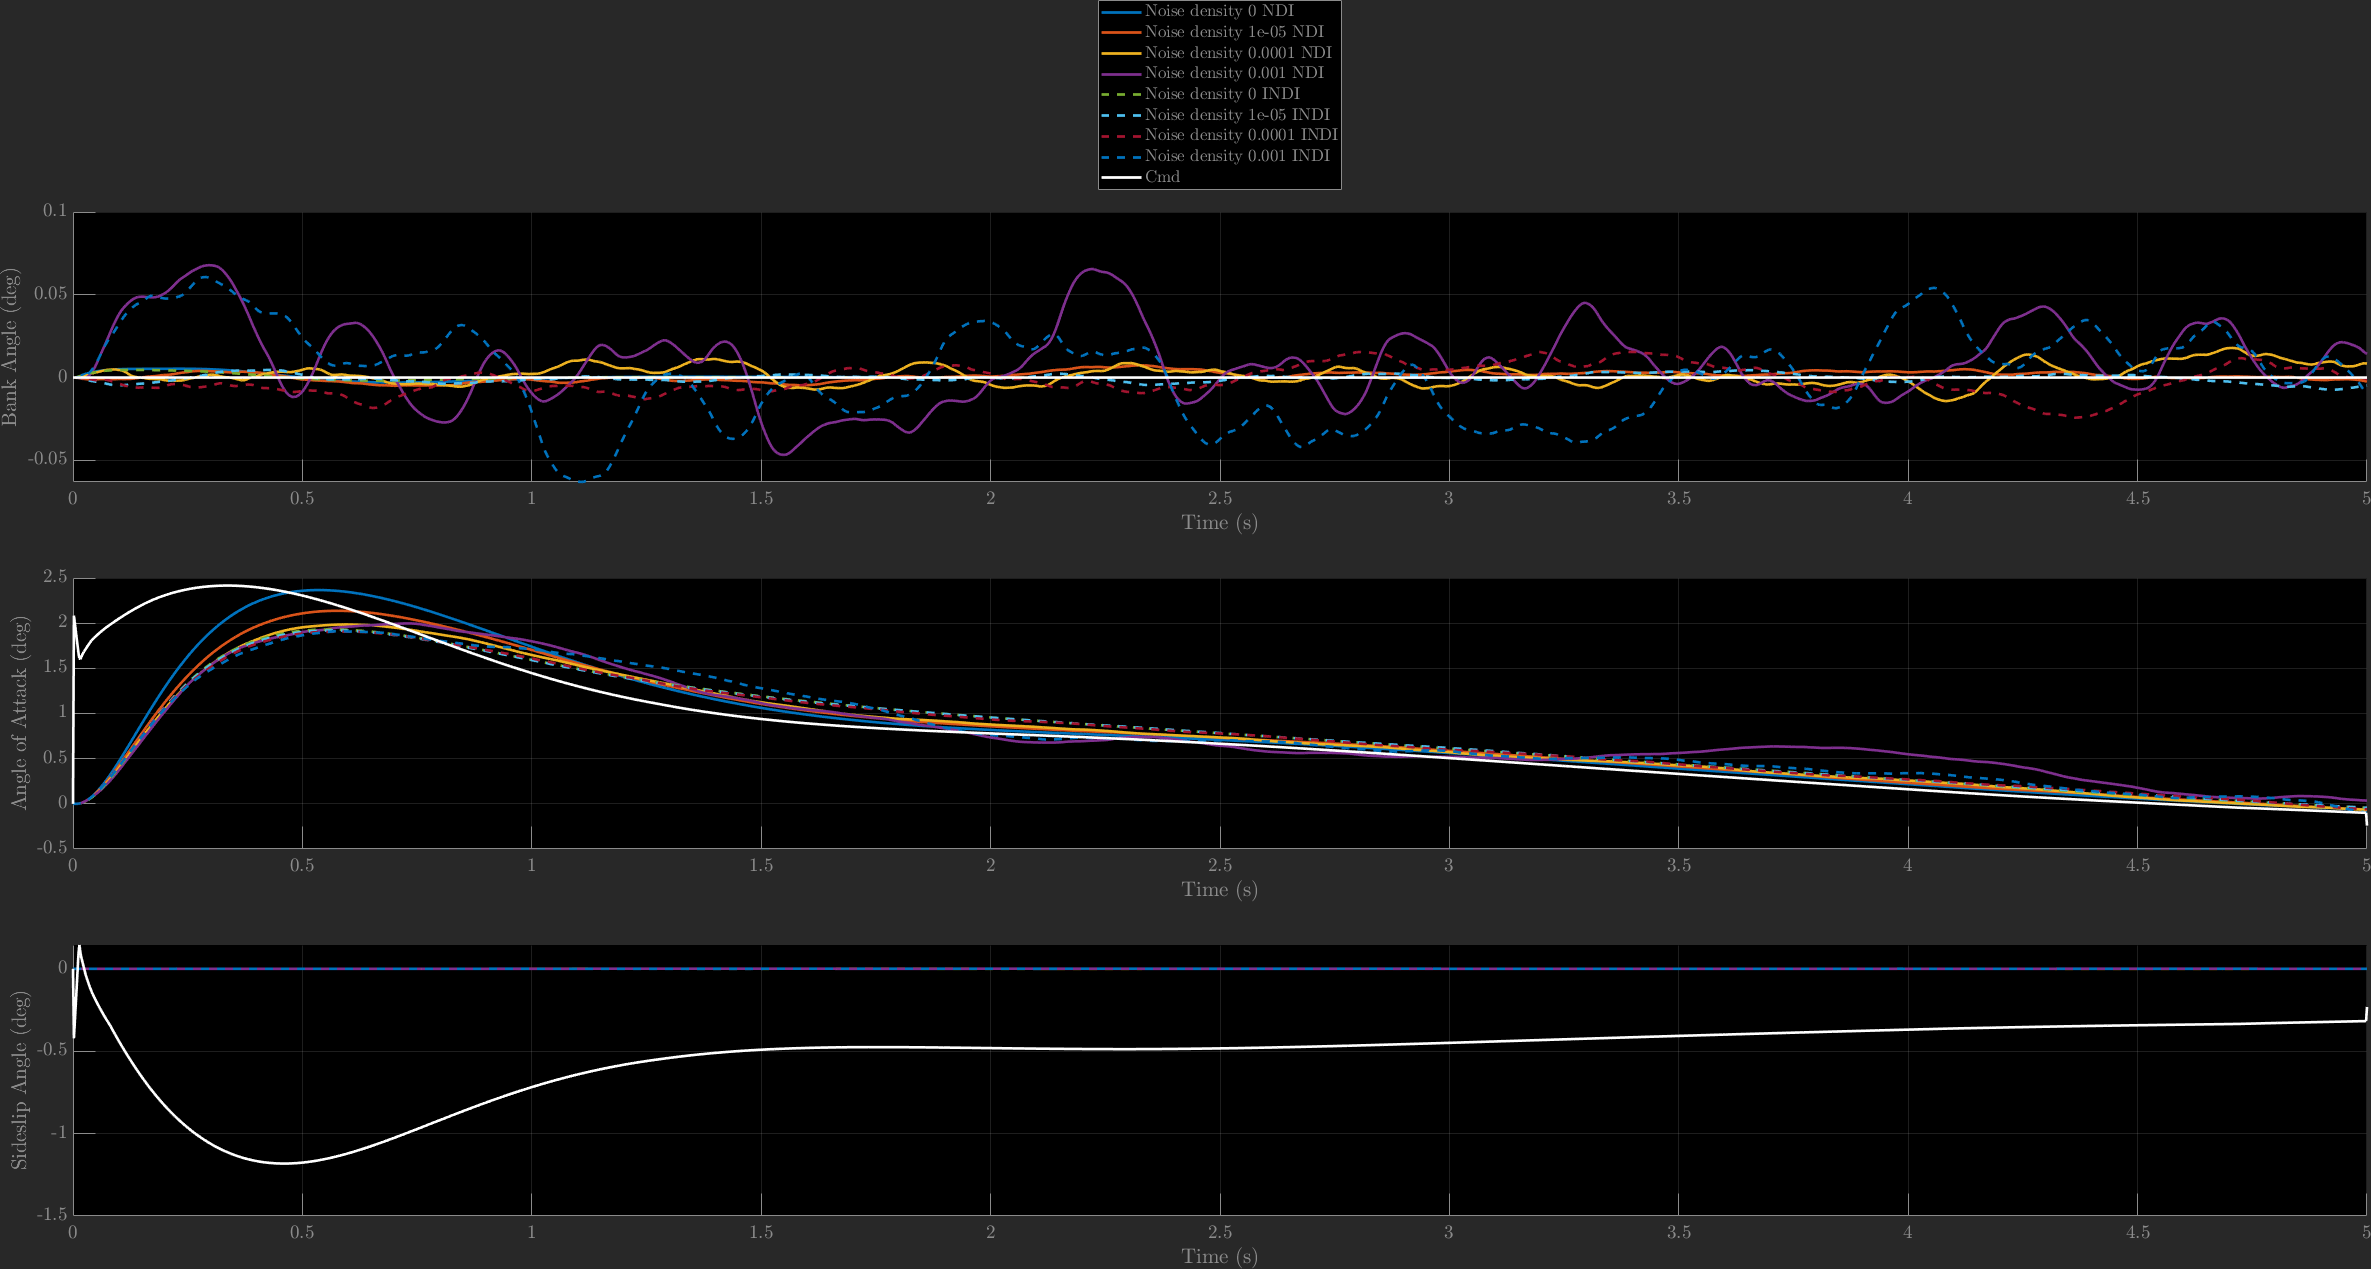
\includegraphics[width=1\textwidth]{Figures/AnglesGuidance.png}
  \caption{Angle tracking results for varying levels of gyroscope noise}
  \label{fig:Angle_Noise}
\end{figure}

\begin{figure}[H]
  \centering
  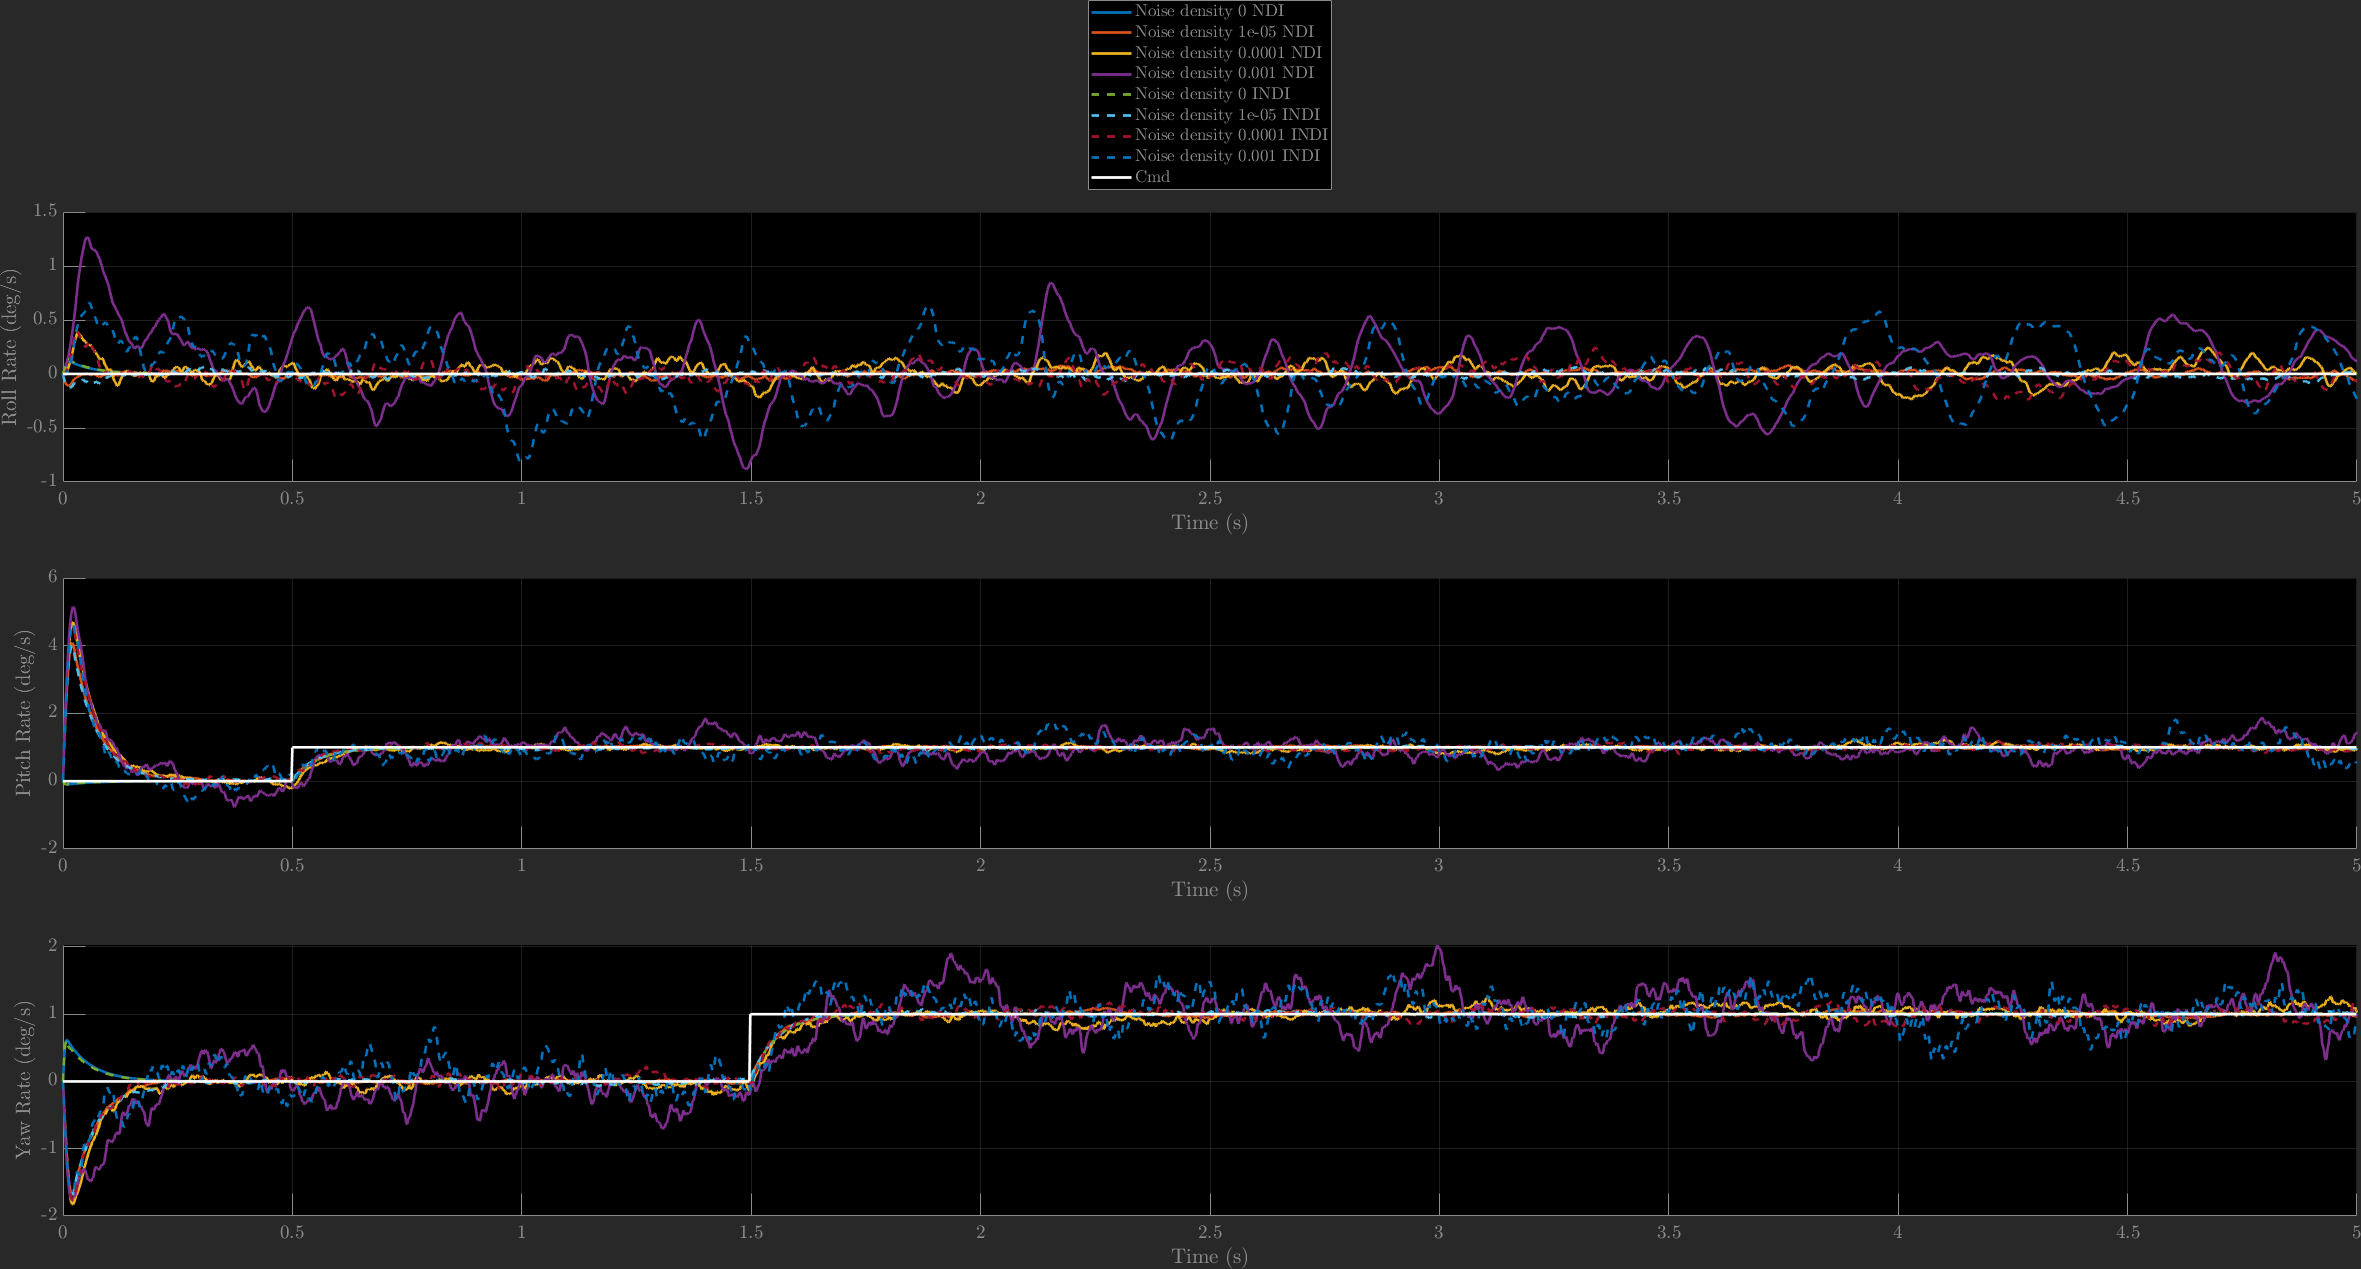
\includegraphics[width=1\textwidth]{Figures/AngularAccelRate.png}
  \caption{Angular rate tracking results for varying levels of gyroscope noise}
  \label{fig:Angular_Rate_Noise}
\end{figure}

\begin{figure}[H]
  \centering
  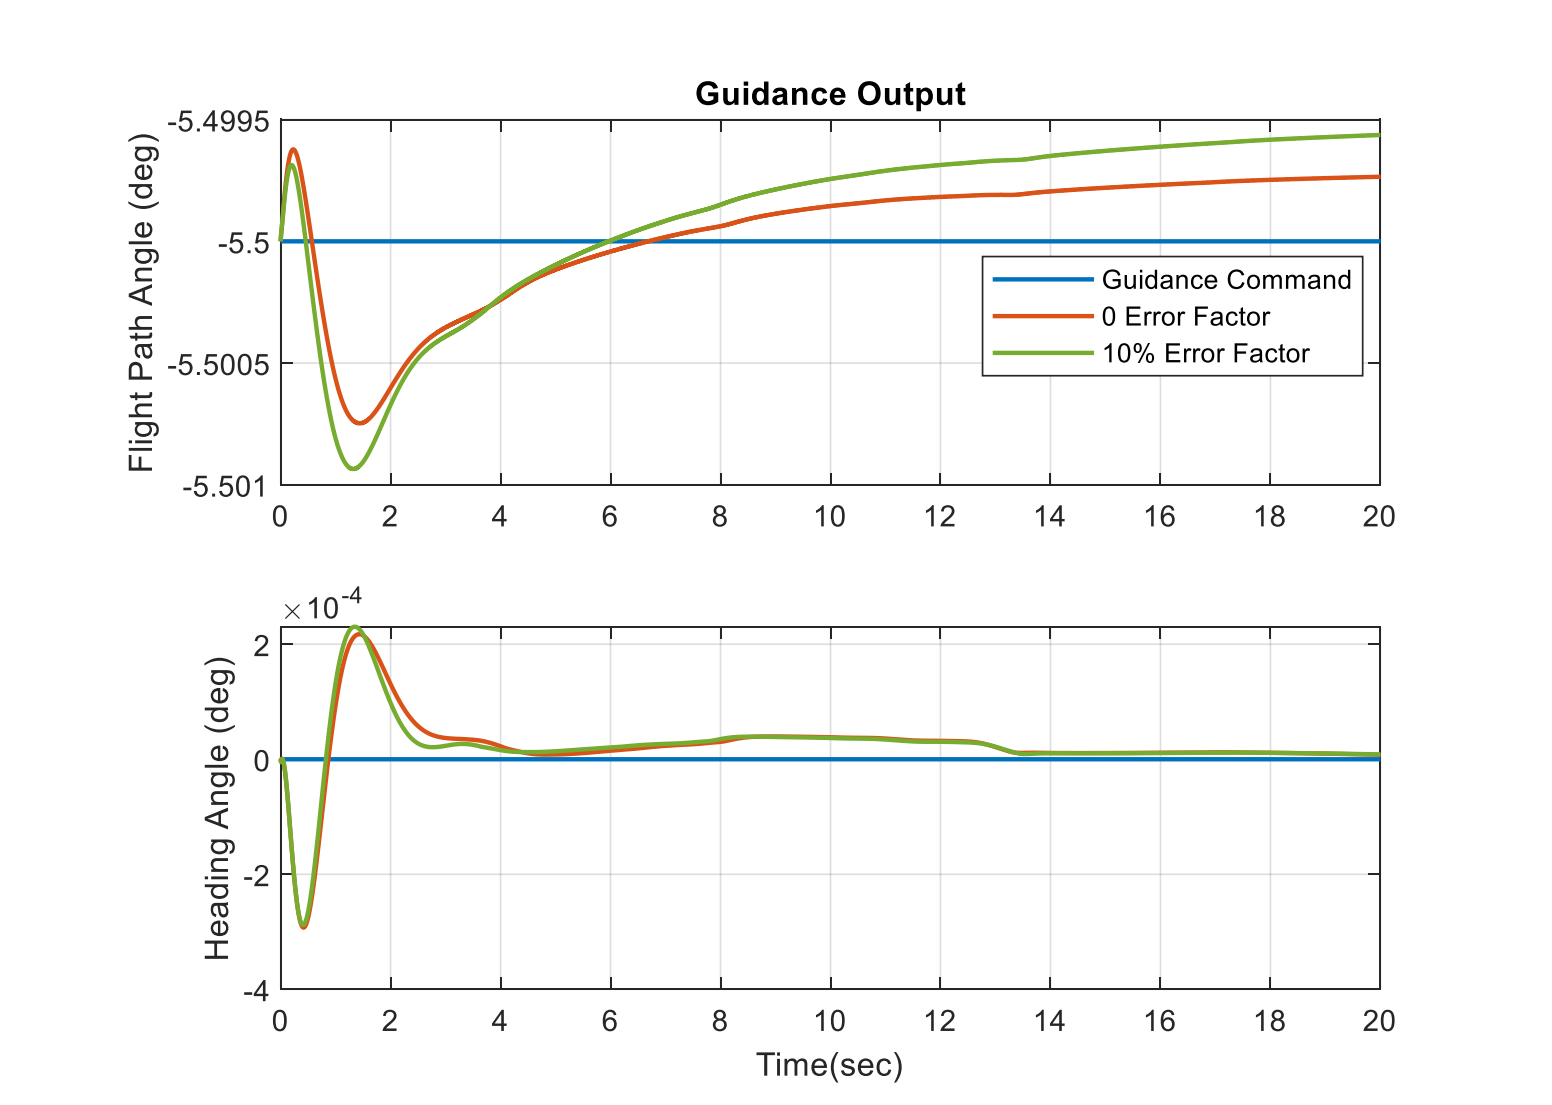
\includegraphics[width=1\textwidth]{Figures/NDI_Parameter_Uncertainty.png}
  \caption{Results of the modelling uncertainty test for the NDI controller [5]}
  \label{fig:Param_Uncertainty}
\end{figure}

\subsection{Control Saturation Testing}
Understanding when the controller will saturate based on a given input is important when designing guidance system that will be providing said inputs. If the control design is such that the actuators do saturate when given commands that would be seen common in real applications, methods must be implemented to help mitigate saturation. Control saturation will limit the guidance system's ability to steer the vehicle to a desired point on a planet's surface, and will place more emphasis on mission planning to ensure that the ADEPT is being inserted into the atmosphere in a location that allows it to reach it's target destination within the constraints of the guidance and control systems. Simulations were ran providing ramp inputs as the flight path angle and heading commands to see if the controller would saturate. The figures below show the that the control law is able to track the given ramp input on flight path angle, and while the control actuators do saturate, it is only for a brief moment.

\begin{figure}[H]
  \centering
  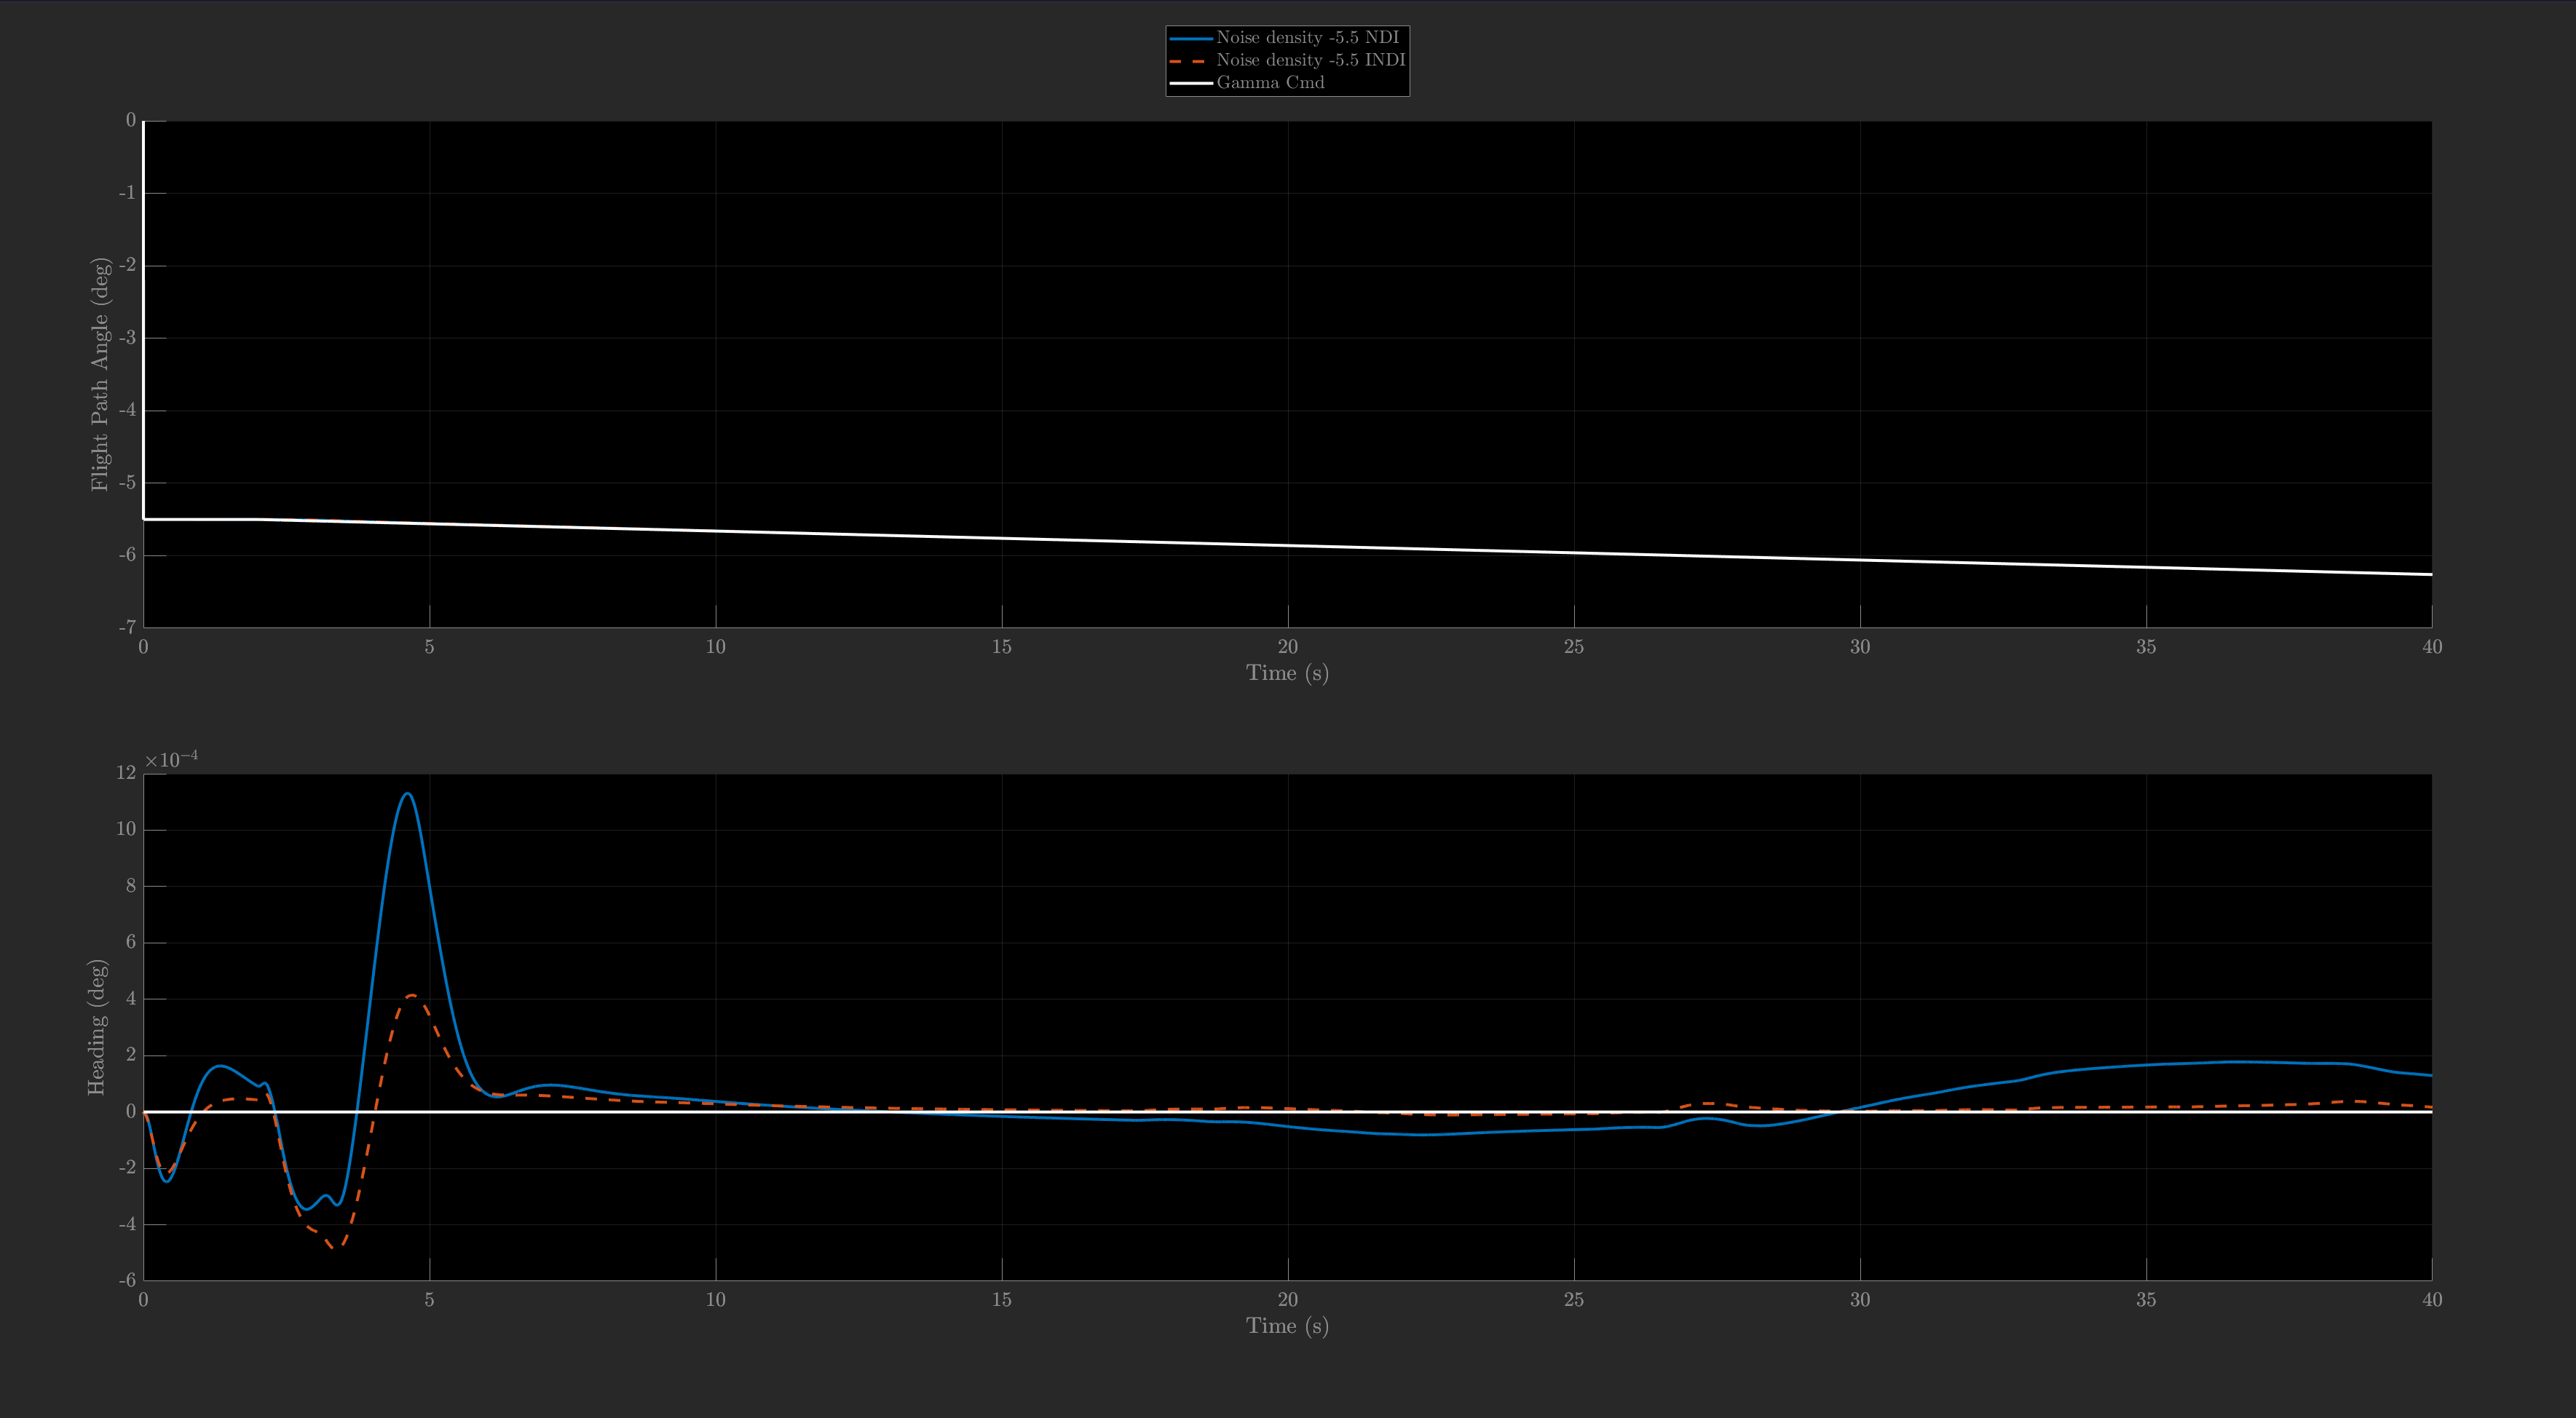
\includegraphics[width=1\textwidth]{Figures/GammaCommand.png}
  \caption{Ramp input given to the flight path angle in one test case}
  \label{fig:GammaCmd}
\end{figure}
\begin{figure}[H]
  \centering
  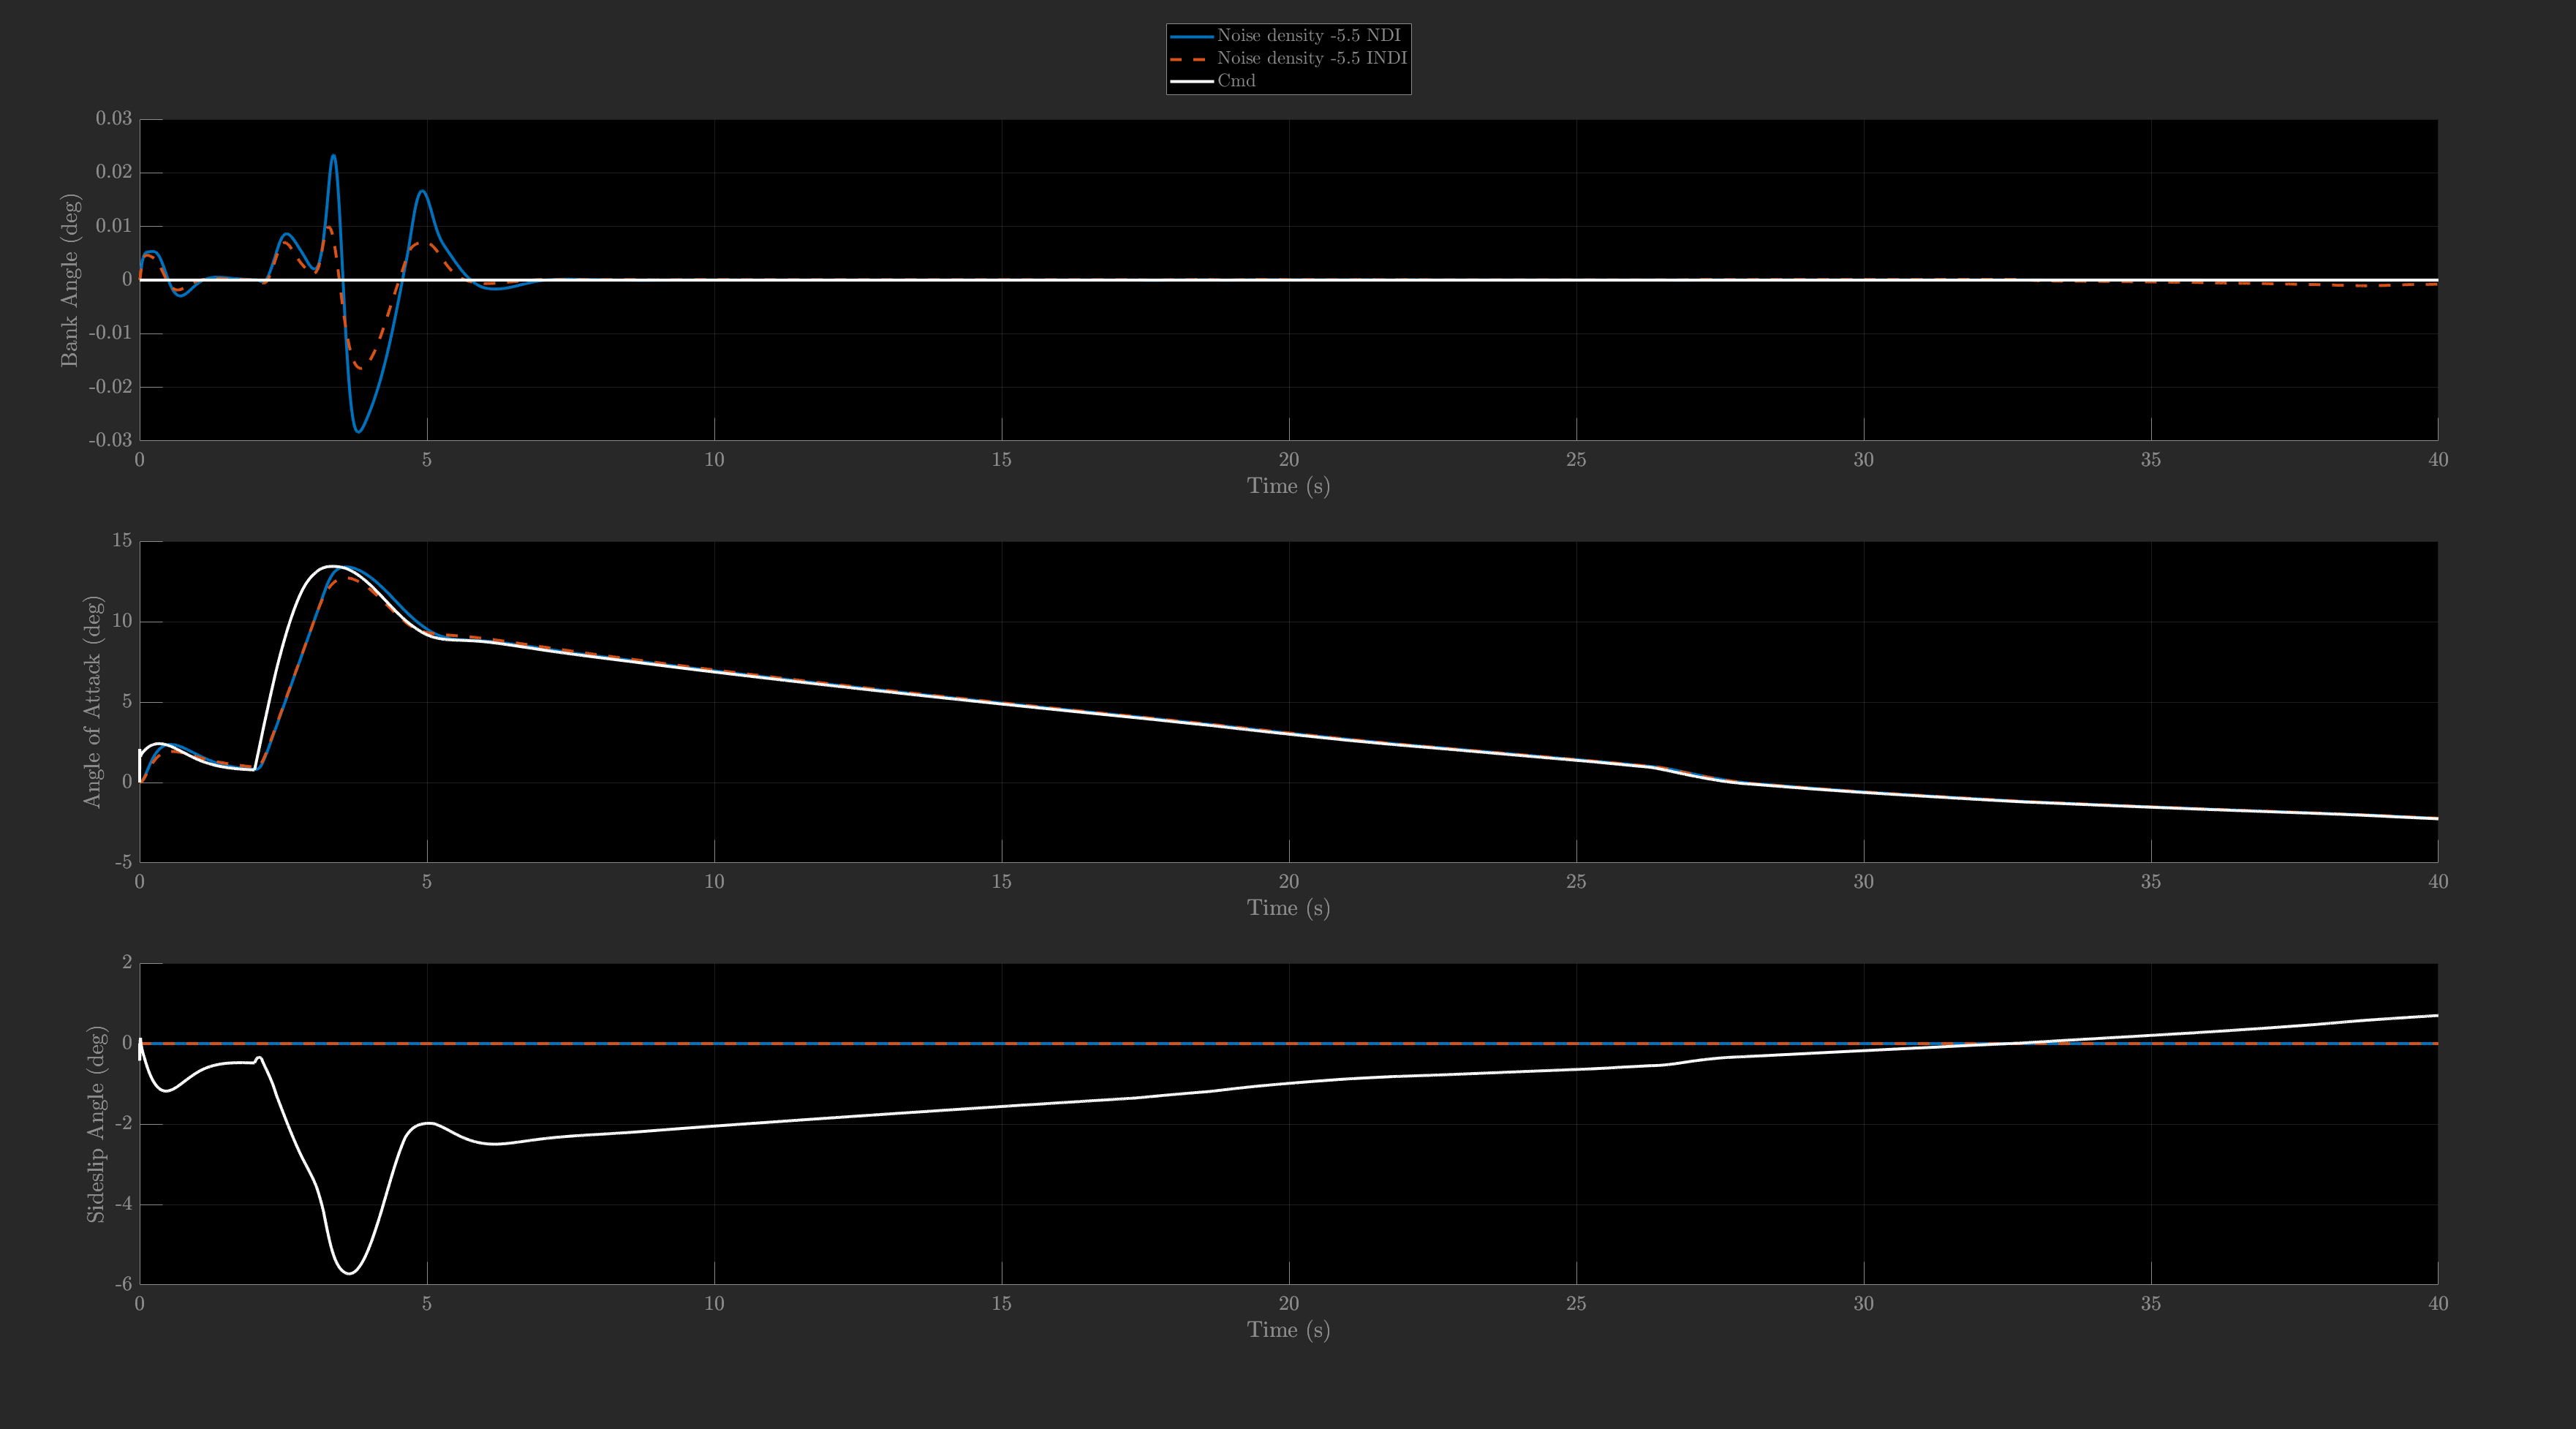
\includegraphics[width=1\textwidth]{Figures/GammaCommandAngles.png}
  \caption{Response of body angles to the input command}
  \label{fig:GammaCmdAng}
\end{figure}
\begin{figure}[H]
  \centering
  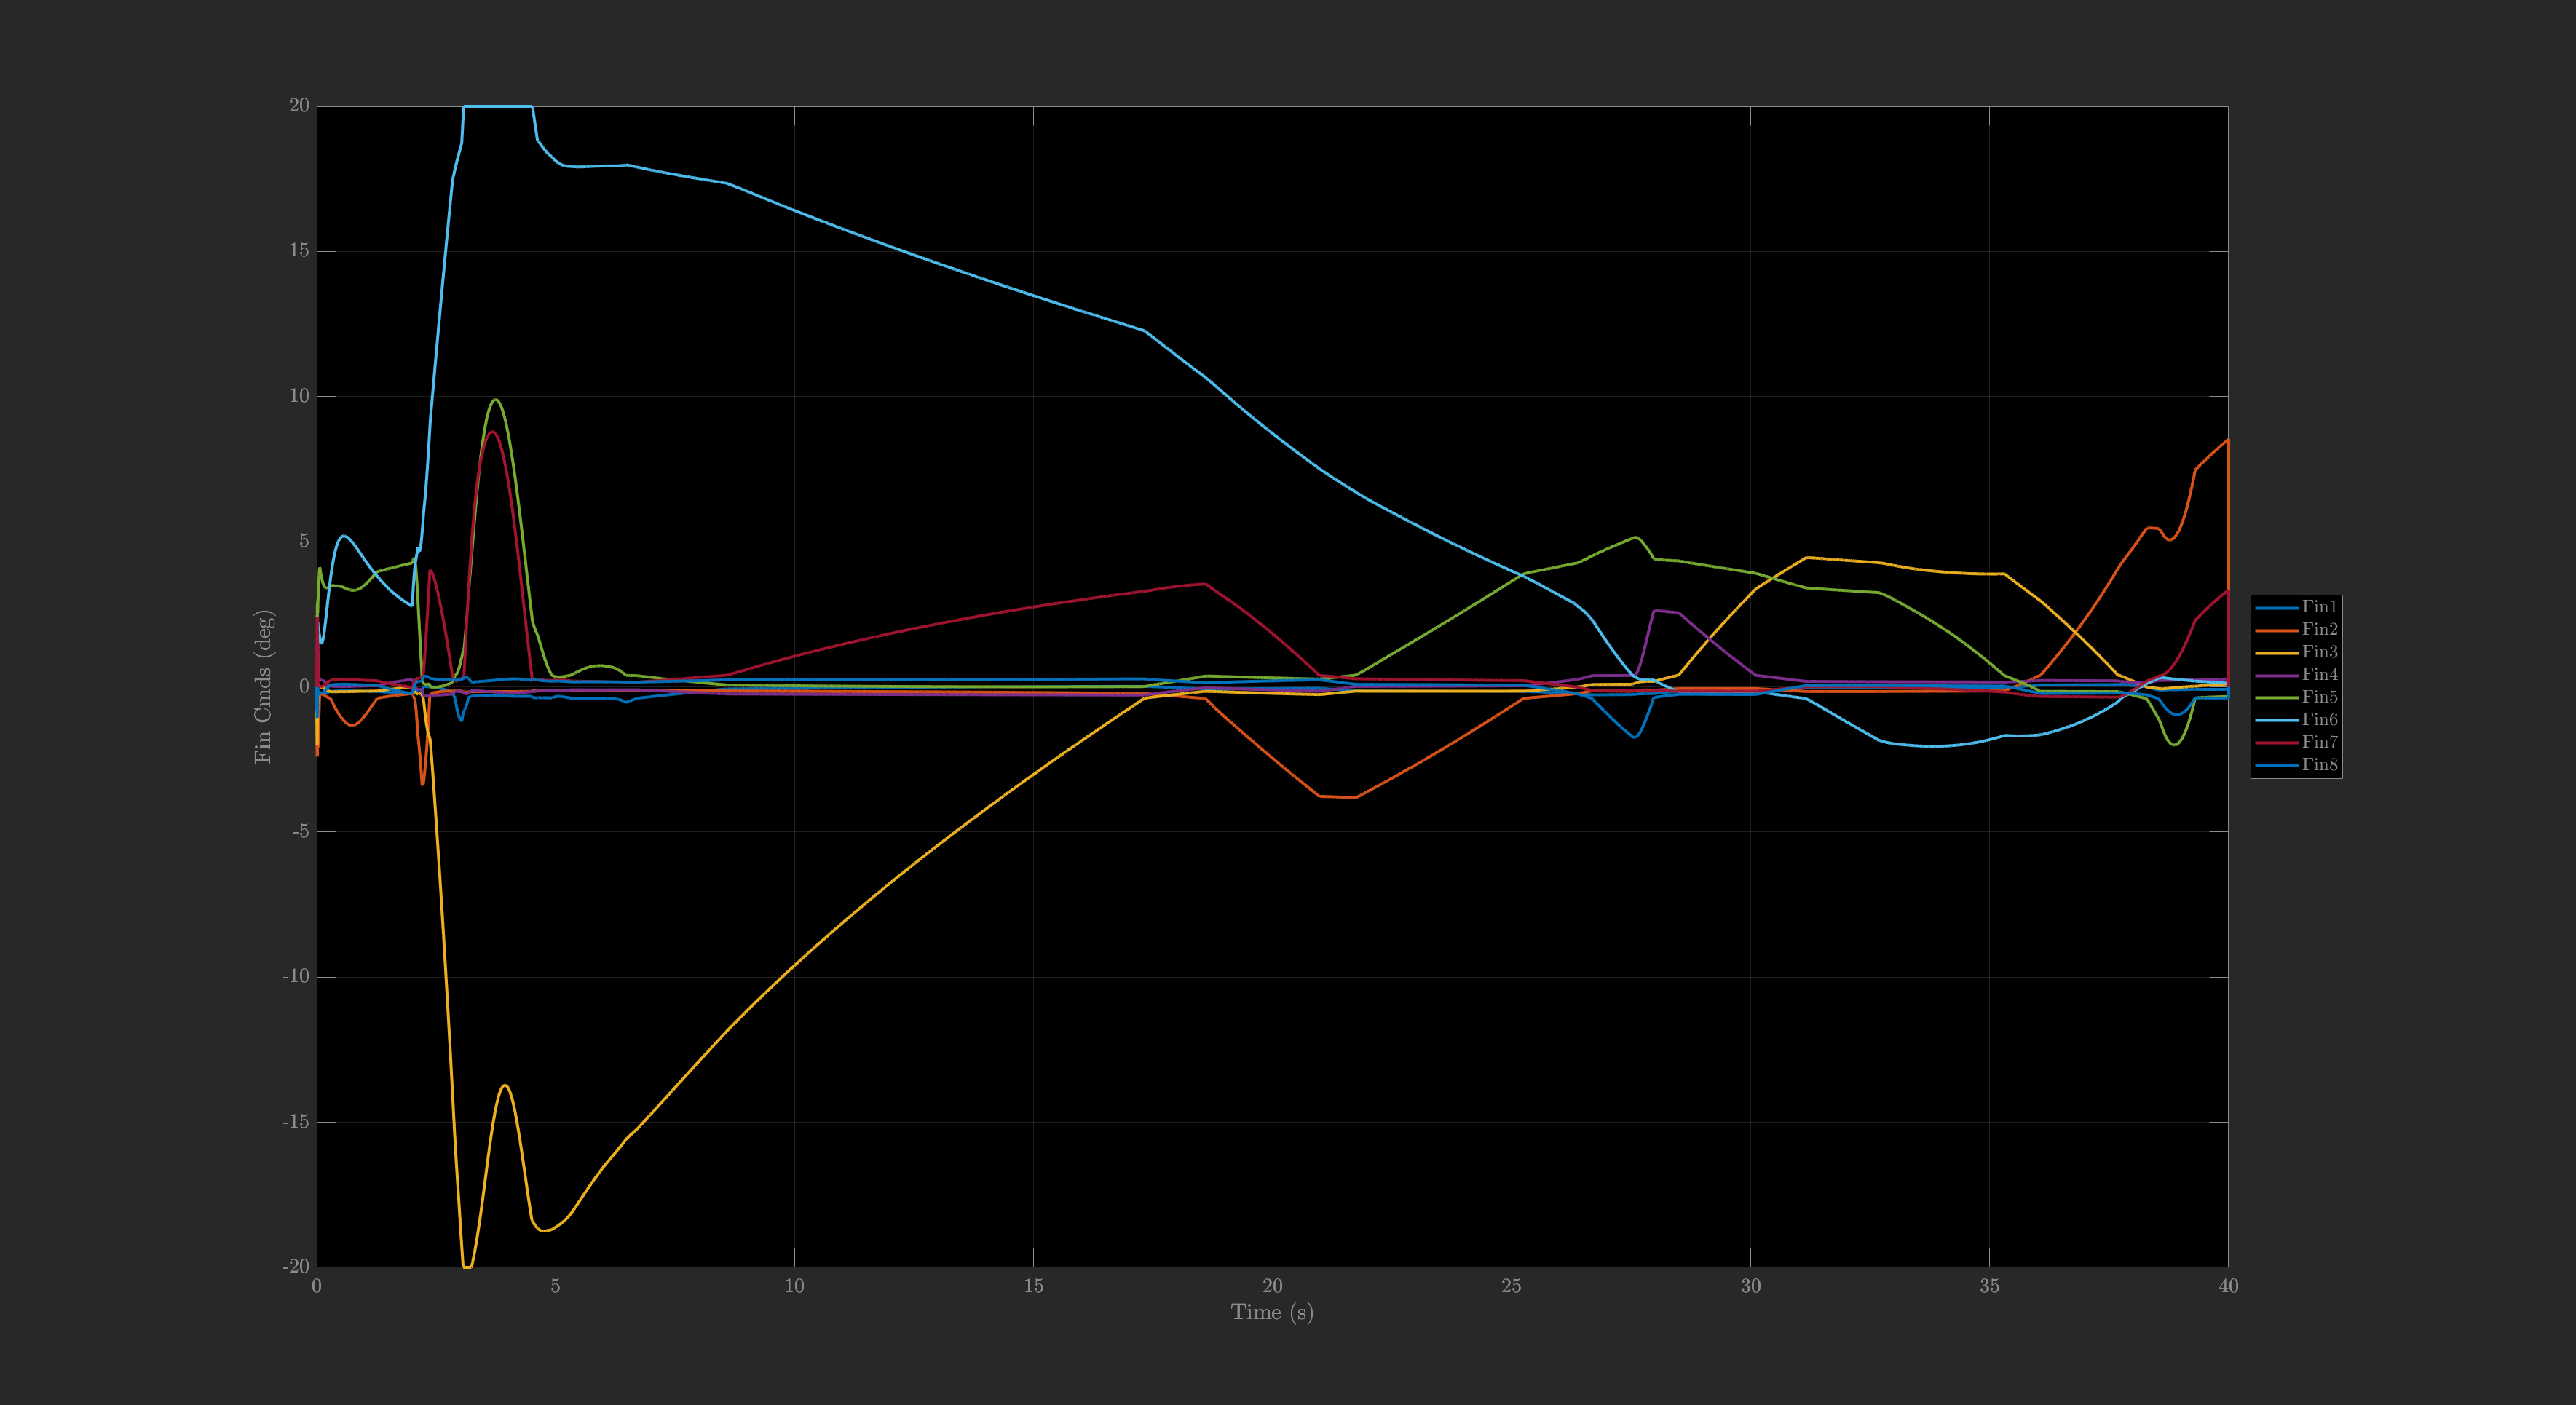
\includegraphics[width=1\textwidth]{Figures/GammaCommandINDIFinDeflect.png}
  \caption{Control surface deflections for the INDI controller}
  \label{fig:GammaCmdFin}
\end{figure}

\subsection{Computational Fluid Dynamics Analysis}
The Computational Fluid Dynamics simulations conducted in [5] only considered hypersonic speeds, therefore the aerodynamic tables were created at a speed of Mach 10 under the assertion that aerodynamic properties did not change much between above roughly Mach 5 [5]. Since the original simulation files for the CFD analysis done in [5] as well as the solid model of the vehicle used in the simulation were no longer available, a new model of the ADEPT RV was created and new CFD simulations must be ran for the entire range of expected Mach numbers down to low supersonic. The solid model of the ADEPT RV main body and flaps was constructed using the SOLIDWORKS computer aided design (CAD) software suite. The remade model including the control surface fins can be seen in the figure below.

\begin{figure}[H]
  \centering
  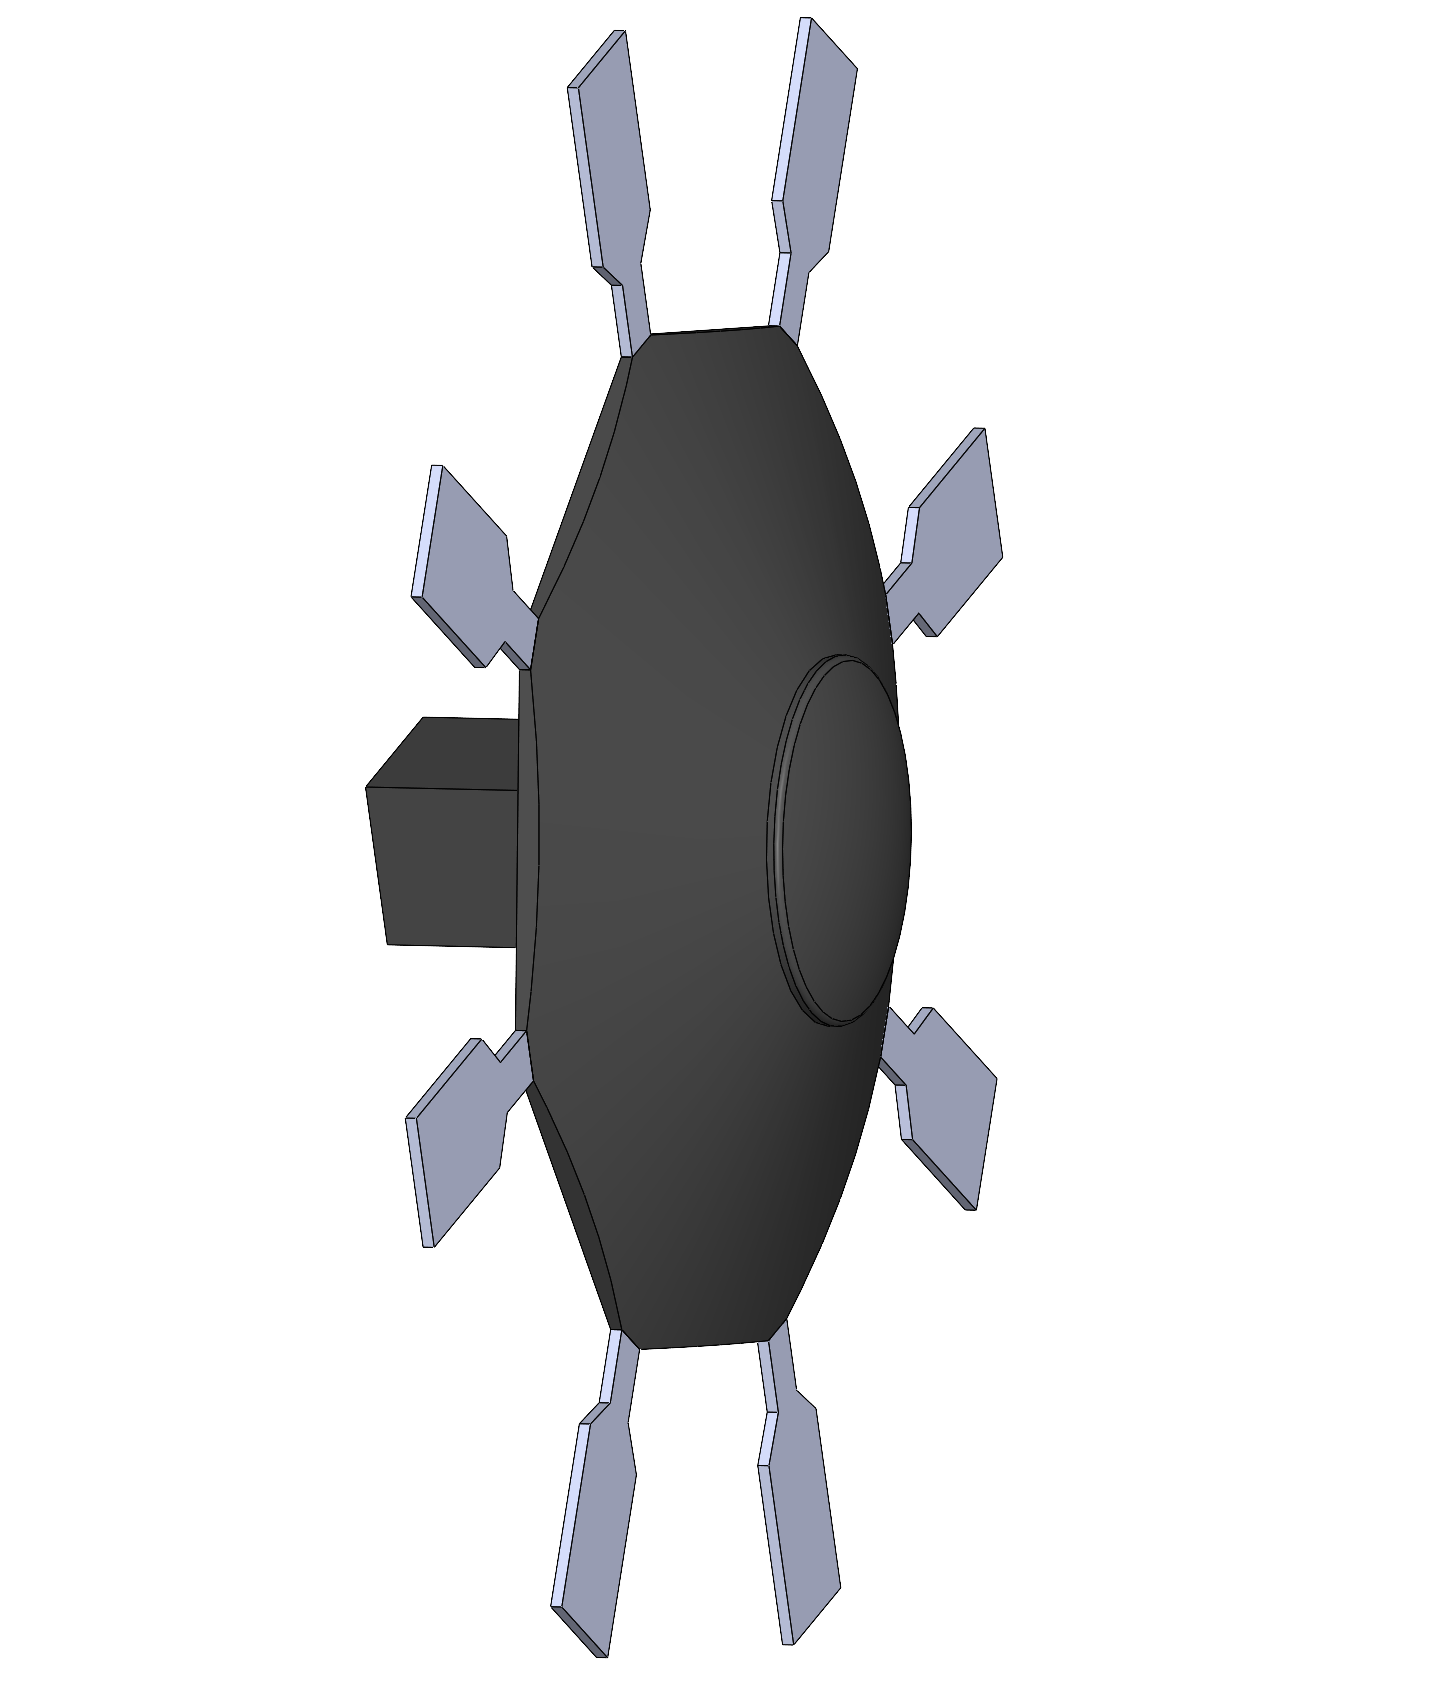
\includegraphics[height=0.5\textwidth]{Figures/ADEPT_CAD.png}
  \caption{CAD Model of ADEPT to be used in CFD simulation}
  \label{fig:DONG}
\end{figure}

\begin{figure}[H]
  \centering
  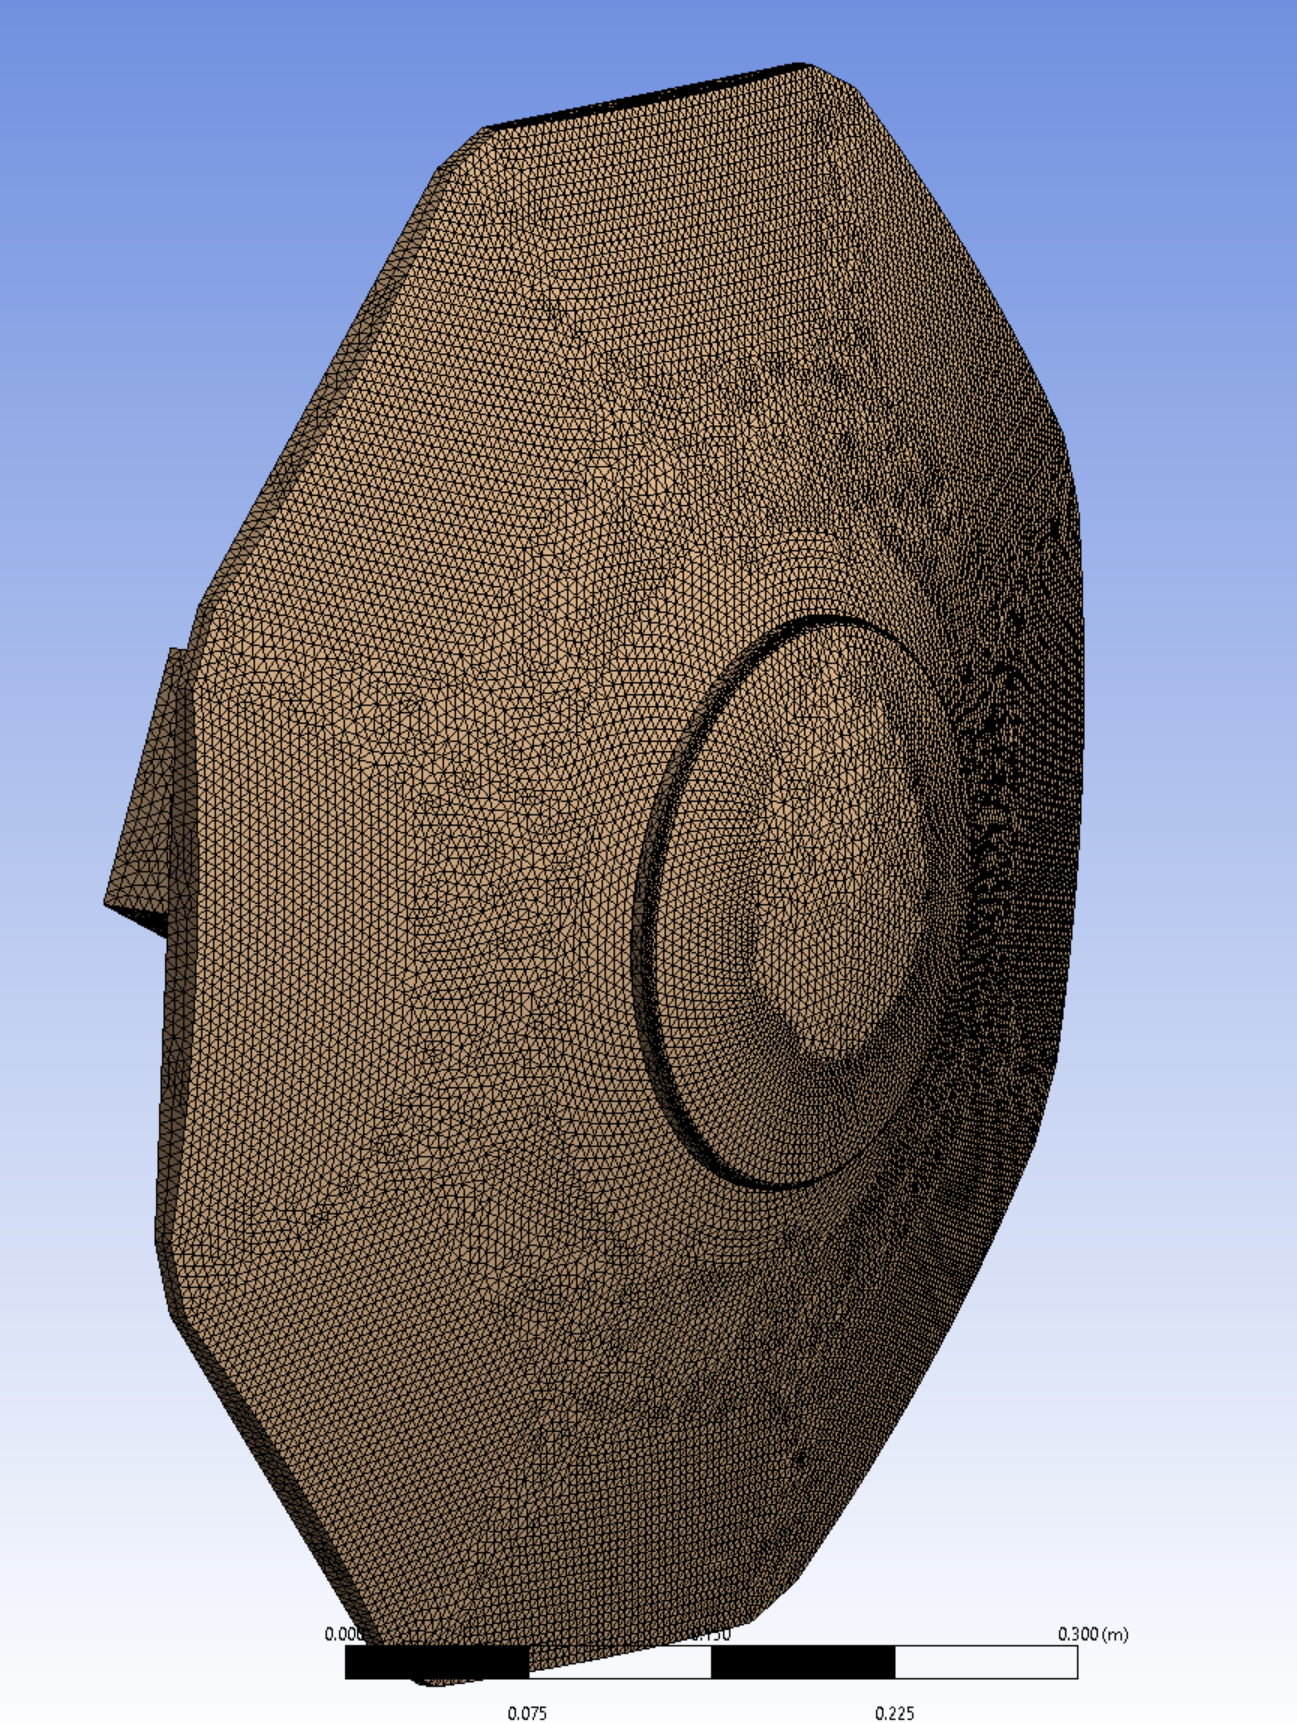
\includegraphics[width=0.5\textwidth]{Figures/ADPEPT_Body_Meshed.png}
  \caption{Meshed ADEPT body in ANSYS Fluent}
  \label{fig:Mesh}
\end{figure}

\begin{figure}[H]
  \centering
  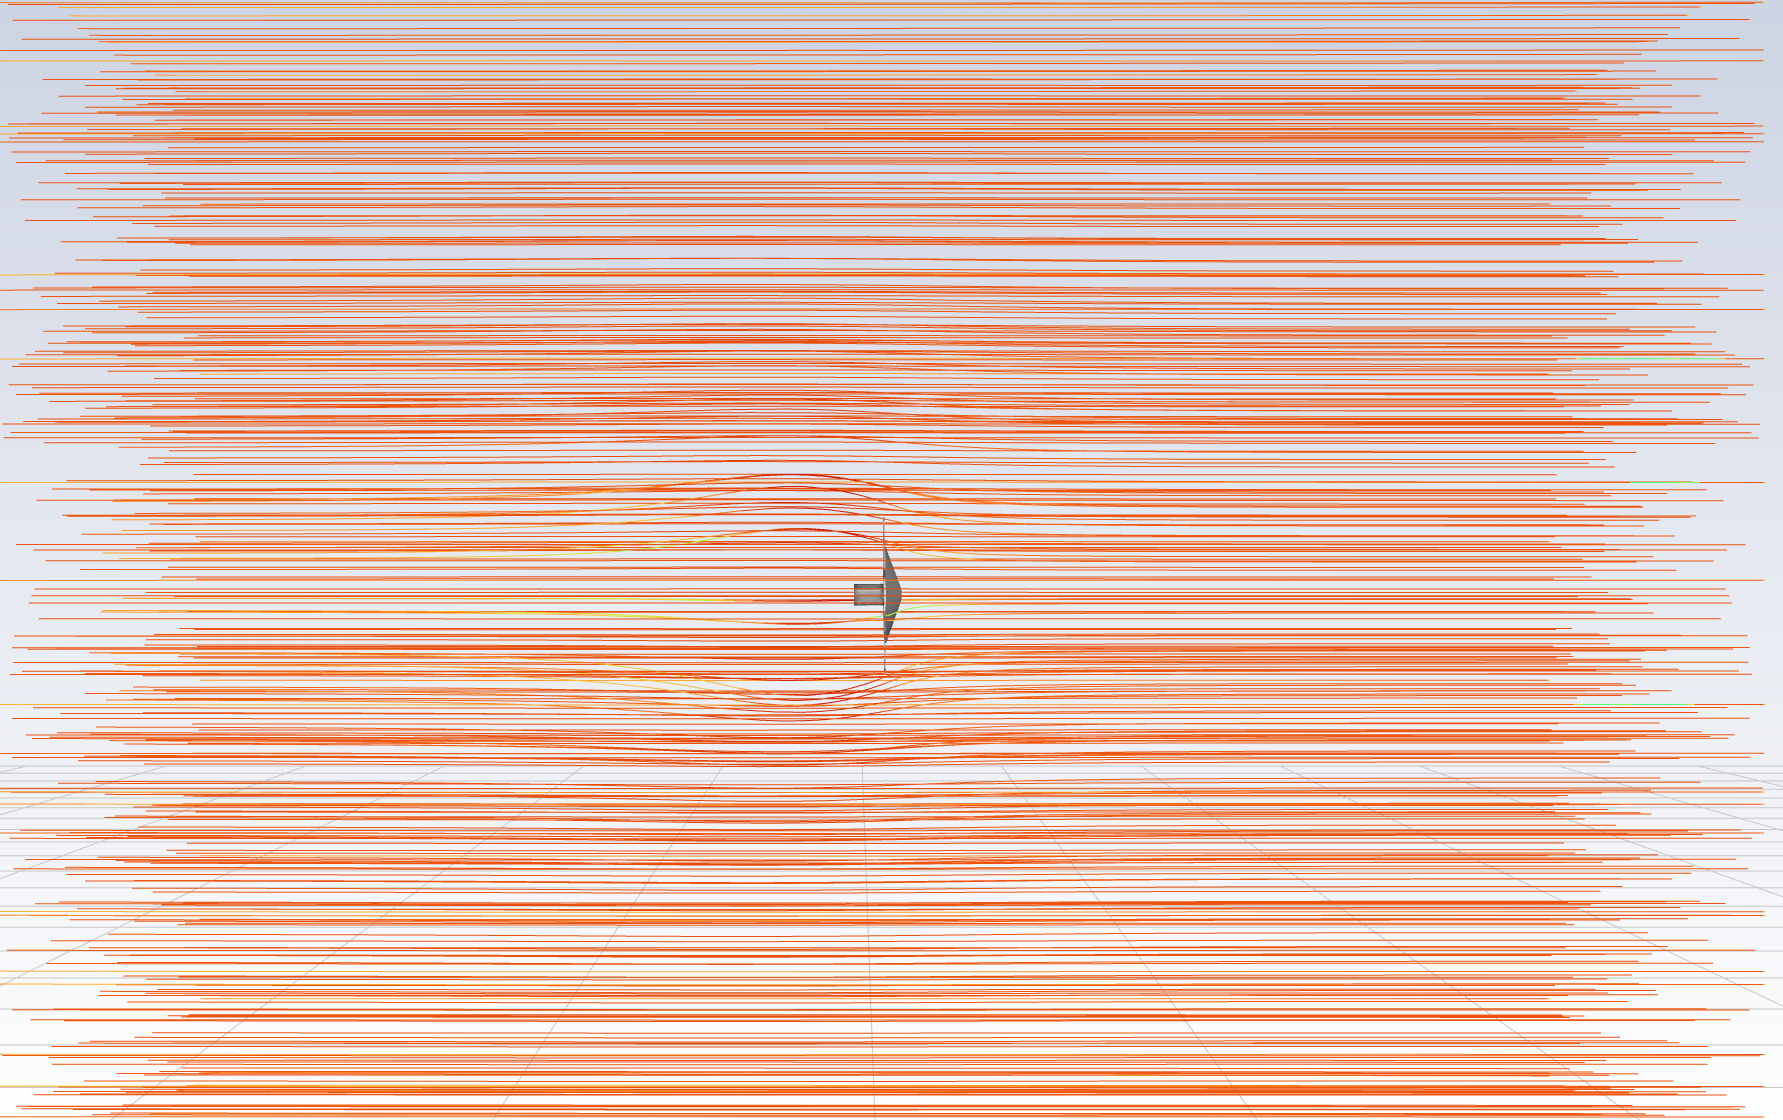
\includegraphics[width=0.75\textwidth]{Figures/ADEPT_In_CFD.png}
  \caption{Meshed ADEPT body in ANSYS Fluent}
  \label{fig:CFD}
\end{figure}

\section{Current Progress}
Currently, work is being done attempting to generate new aerodynamic tables using ANSYS Fluent CFD software. Progress has been slower than ideal due to the learning curve of both Fluent and SOLIDWORKS CAD software, but simulations are currently being conducted to populate the tables. Once the tables are populated, they will be used in the simulation and performance benchmarked against the previous aerodynamic tables. Tables going down to speeds in the low supersonic regime should provide adequate data to be used in the simulation with the guidance system guiding the vehicle to a point on the planet's surface. The report will be updated with CFD results and plots of the aerodynamic coefficient surfaces once all simulation runs are complete.

At the moment, control actuator saturation seems to not be a concern, but it is as of yet unknown the level of command that will be generate by the guidance algorithm. Research has been done into the pseudo-control hedging scheme, outlined in [23], with a rough algorithm implemented already should the need arise once the guidance work progresses. Progress has also been hindered by an apparent bug that occurs when running the simulation for long times of flight, as would be seen when attempting to guide the vehicle to the ground from the upper atmosphere. The cause of the bug is currently unknown, but work is being done to figure out the issue. An example of the simulation output for longer flight times can be seen in the figure below. Significant time has been put into commenting and refactoring code in tandem with the other work presented in this paper so far, which should help to quickly find and fix and bugs that may present themselves in the future. The issue may also be caused by the aerodynamic tables assuming the speed will always be hypersonic, which is not the case for long flight times. Results will be compared when the new aerodynamic tables are added to the simulation.

\begin{figure}[H]
  \centering
  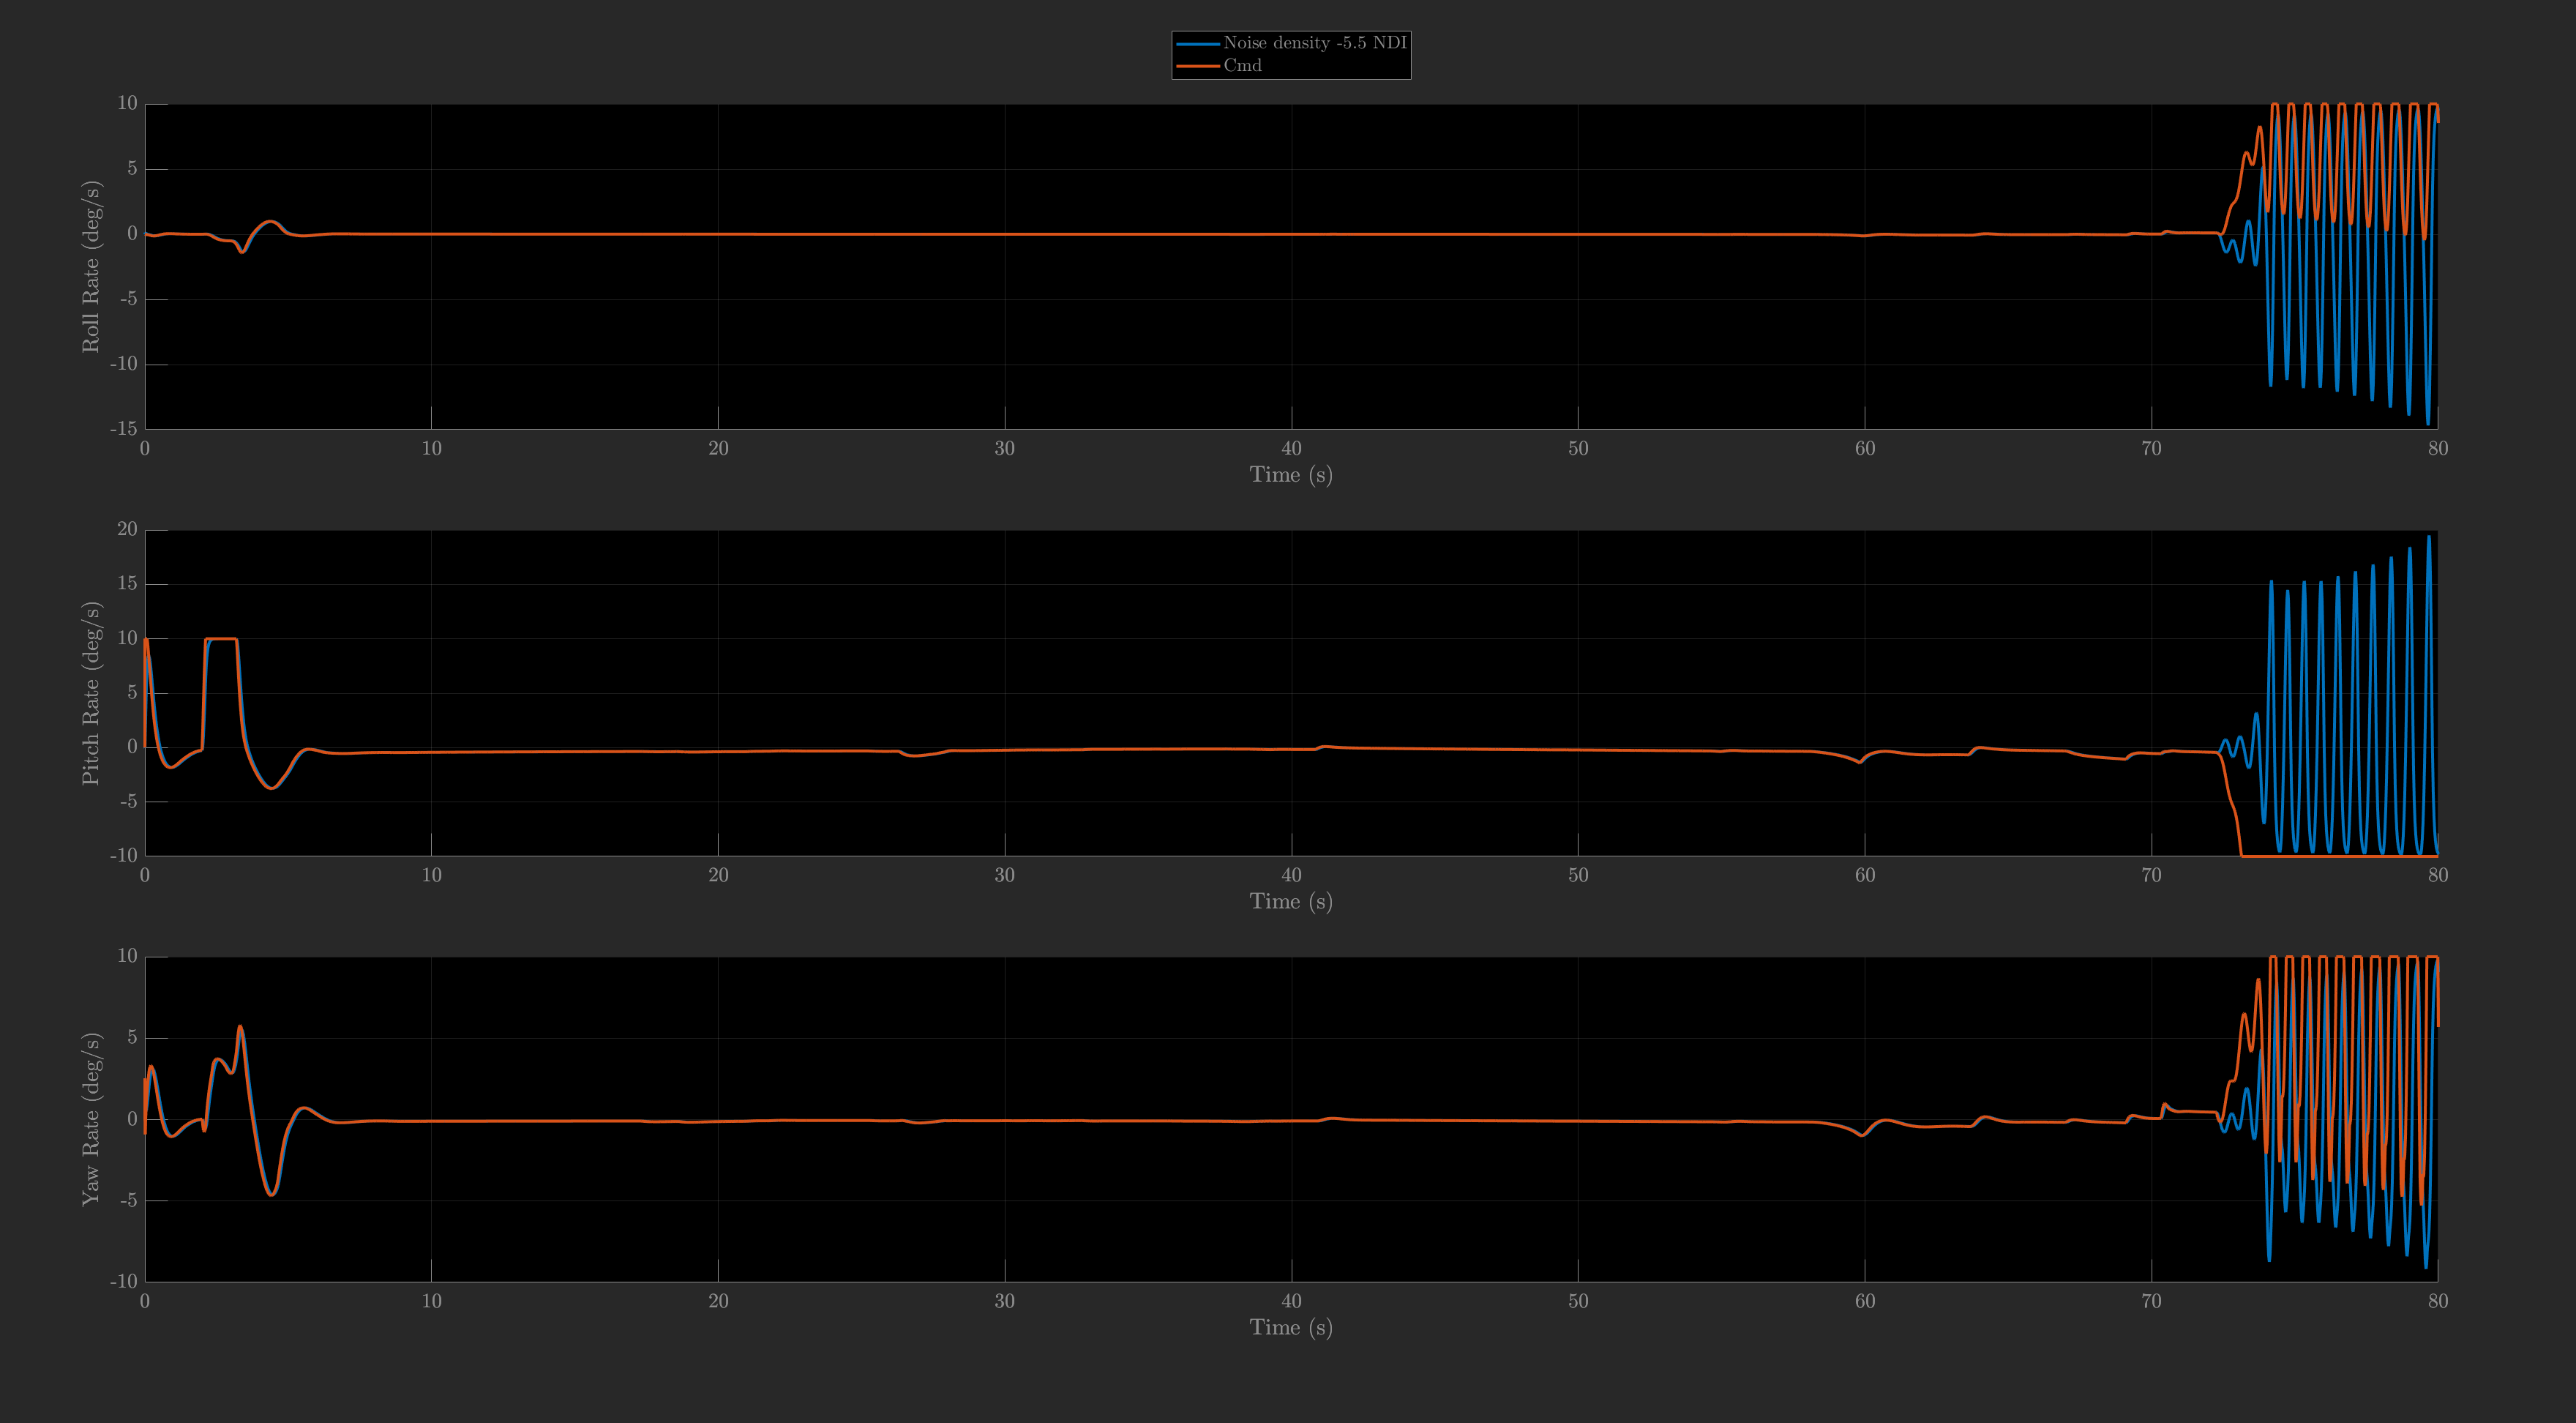
\includegraphics[width=1\textwidth]{Figures/bug.png}
  \caption{Figure illustrating odd simulation behavior for long flight times}
  \label{fig:bug}
\end{figure}

\nocite{*}
\bibliography{sample}
\end{document}
